\documentclass[11pt, a4paper]{article}

% --- PACKAGES ---
\usepackage[margin=1in]{geometry}
\usepackage{amsmath}
\usepackage{graphicx}
\usepackage{booktabs} % For professional tables
\usepackage{amssymb} % For symbols like \mathbb{R}
\usepackage{amsfonts}
\usepackage{bm} % For bold math symbols
\usepackage{amsthm} % For theorem-like environments
\usepackage{enumitem} % For customized lists

% --- DOCUMENT SETUP ---
% We define the title elements manually inside the 'titlepage' environment
% \title{Technical Reference Note: \\ A Modern Framework for Smoothing in Additive Models}
% \author{Personal Reference Document}
% \date{\today}

\newtheorem{definition}{Definition}
\newtheorem{theorem}{Theorem}
\newtheorem{lemma}{Lemma}

% --- BEGIN DOCUMENT ---
\begin{document}

\begin{titlepage}
 \centering % Center everything on the page
 
 \vspace*{1cm} % Add some space at the top
 
 {\Huge \bfseries Splines Overview}
 
 \vspace{2cm} % Space between title and image
 
 % --- IMAGE ---
 % Make sure the image file 'spline-ducks.png' is in the same directory
 % as your .tex file. Adjust width as needed.
 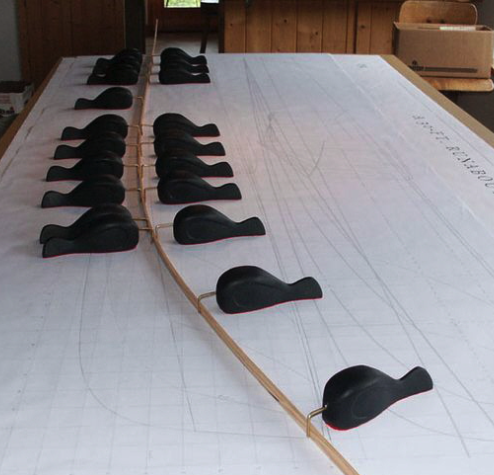
\includegraphics[width=0.6\linewidth]{spline-ducks.png}
 
 \vfill % Pushes the content below to the bottom of the page
  
 \vspace{1cm}
 
 {\large \today}

\end{titlepage}

\tableofcontents
\newpage
\section{Intro to Splines and Smoothing}
\subsection{1.1 The Physical Analogy: The Draftsman's Spline}
The term ``spline'' originates from a tool used by draftsmen: a long, thin, flexible strip of wood. To draw a smooth curve through a set of points, they would place lead weights (``ducks'') at the required locations and bend the strip against them. The strip naturally settles into a shape that minimizes its total bending energy. This physical concept is mathematically equivalent to minimizing the integrated squared second derivative of a function, $\int [f''(x)]^2 dx$, which is a measure of its total ``wiggliness''.


\subsection{1.2 Basis Functions}
Instead of defining a single complex function, we can construct it from a set of simple, known ``building block'' of functions, $b_k(x)$, called a \textbf{basis}. The final complex curve $f(x)$ is a weighted sum of these blocks:
\[ f(x) = \sum_{k=1}^{K} \beta_k b_k(x) \]
The smoothness of $f(x)$ is determined by the values of the coefficients $\beta_k$. If adjacent coefficients are very different, the curve will be wiggly. If they are similar, it will be smooth. ``Penalizing wiggliness'' therefore becomes equivalent to penalizing large differences between adjacent coefficients.
\begin{figure}
 \centering
 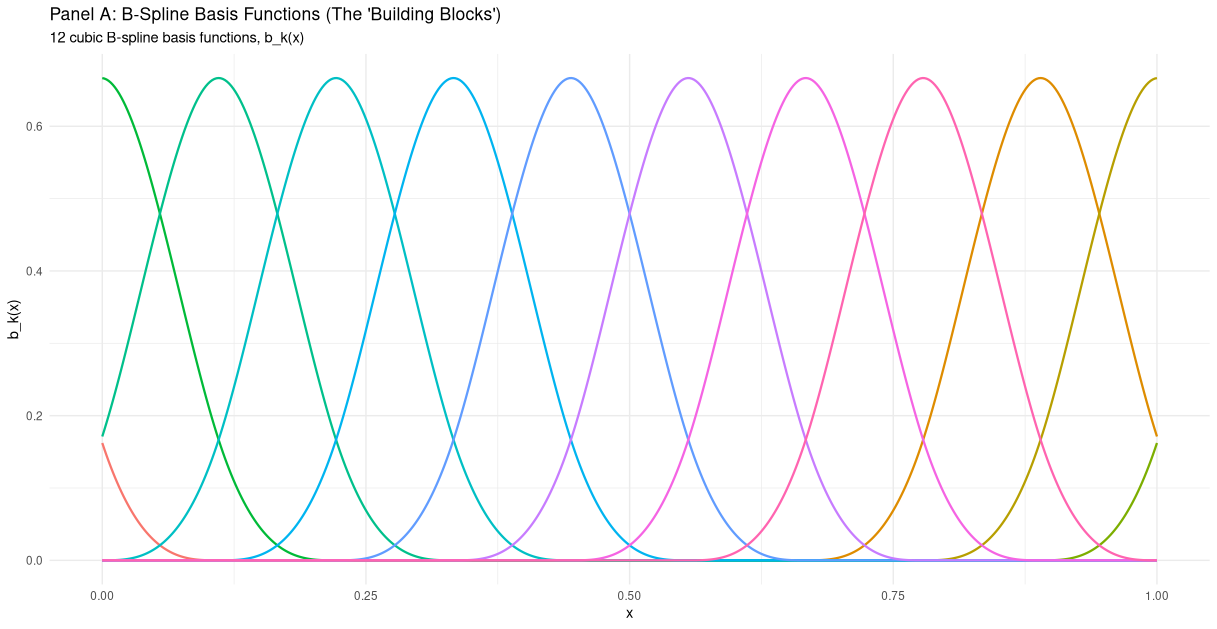
\includegraphics[width=\linewidth]{b-splines.png}
 \caption{B Spline Basis Functions}
 \label{fig:enter-label}
\end{figure}

\begin{figure}
 \centering
 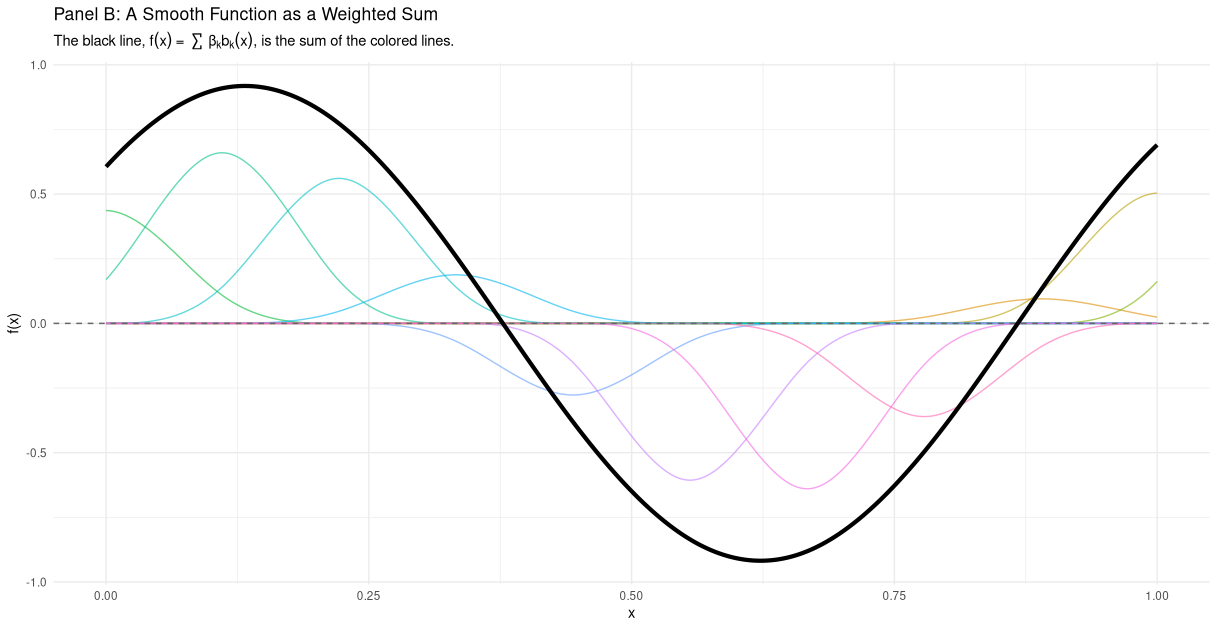
\includegraphics[width=1\linewidth]{weighted.png}
 \caption{Weighted Basis Functions}
 \label{fig:enter-label}
\end{figure}

\newpage
\section{Knot placement and Penalized Splines}
The development of penalized splines was largely motivated by the inherent difficulties encountered with earlier spline methodologies, particularly concerning the selection of knots and the risk of overfitting when using flexible basis expansions. 

\subsection{2.1 The Limitations of Manual Knot Placement: Subjectivity, Misspecification, and Instability}
In traditional spline regression, the function is constructed by joining polynomial pieces at specific points known as knots. The number and location of these knots are critical as they dictate the flexibility of the spline. If too few knots are used, the spline may be too stiff to capture the true underlying function $\Rightarrow $ underfitting. Conversely, while more knots offer greater flexibility, their improper placement or an excessive number in an unpenalized setting can lead to overfitting.

Manual selection of knots introduces several significant limitations:
\begin{itemize}
 \item \textbf{Subjectivity and Reproducibility:} The choice of knot locations is often subjective, relying on visual inspection of the data or domain expertise. Different analysts, or even the same analyst at different times, might select different knot configurations for the identical dataset. This subjectivity inherently compromises the reproducibility of the model and its findings, which is a fundamental tenet of scientific research. While the goal of employing splines is often to allow the data to determine the functional form without strong parametric assumptions, manual knot selection reintroduces a substantial element of user judgment.

 \item \textbf{Misspecification Bias:} If knots are not placed in regions where the true underlying function exhibits changes in behavior—such as peaks, troughs, or points of inflection—the spline will be unable to adapt to these features adequately. This leads to misspecification bias, where the fitted model systematically deviates from the true function in those regions. For instance, if a function has a sharp peak but no knot is placed near it, the spline will smooth over this feature. The performance of splines is highly dependent on the chosen knot locations. Improper placement can lead to a misrepresentation of the data's inherent structure.

 \item \textbf{Underfitting:} A common issue arising from manual selection is the use of too few knots. This results in a spline that is overly stiff and lacks the necessary flexibility to capture the true complexity present in the data, leading to underfitting. Visualizing this, attempting to fit a complex, oscillating function with only a few knots will inevitably result in a poor representation that misses key variations.

 \item \textbf{Local Overfitting and Instability:} Even if a seemingly reasonable number of knots is chosen, their suboptimal placement can be problematic. For example, clustering knots in relatively flat regions of the function while having too few knots in highly variable (wiggly) regions can lead to the spline fitting noise locally in the over-parameterized segments and underfitting in others. This can result in an unstable overall fit. The sensitivity to knot choices is well-documented; for instance, increasing the number of knots or repeating knots directly impacts the smoothness and local behavior of the spline fit.

 \item \textbf{"Optimal" Knot Placement:} Recognizing these difficulties, considerable research effort was historically dedicated to developing methods for automatically selecting "optimal" knot points. Techniques such as Generalized Cross-Validation (GCV), Akaike's Information Criterion (AIC), or Bayesian Information Criterion (BIC) were employed to guide knot selection. Strategies included placing knots at quantiles of the predictor variable or using domain-specific knowledge. While these automated methods were an improvement over purely manual selection, they often involved significant computational burden, especially if cross-validation was performed over many potential knot sets. Furthermore, they did not fully resolve the issue of pre-specifying the \textbf{number} of knots, which itself influences the optimal locations. 
\end{itemize}
The challenges associated with manual or heuristic knot selection—subjectivity, potential for misspecification and underfitting, and the computational cost of optimization—were significant drivers for the development of penalized spline methods. These modern approaches aim to make the choice of knots, particularly their number and exact locations, far less critical by employing a different strategy: using a sufficiently large number of knots and controlling the model's smoothness via a penalty term.

\subsection{2.2  Overfitting  of  Unpenalized Basis Functions}
To circumvent the difficulties of selecting a small, optimal set of knots, an alternative approach might be to use a very large number of basis functions. This implies using many knots, often placed at regular intervals across the range of the covariate, or even, in the limit of classical smoothing splines, a knot at every unique data point. The rationale is to ensure that the basis is rich enough to capture any potential complexity in the underlying function. However, if these basis functions are used in a standard regression framework without any form of regularization (i.e., unpenalized), a severe problem known as overfitting arises.

Consider the standard linear model formulation $\mathbf{y} = \mathbf{X}\boldsymbol{\beta} + \boldsymbol{\epsilon}$, where $\mathbf{y}$ is the vector of observed responses, $\mathbf{X}$ is the $n \times K$ model matrix derived from $K$ basis functions evaluated at $n$ observation points, $\boldsymbol{\beta}$ is the vector of $K$ coefficients to be estimated, and $\boldsymbol{\epsilon}$ is the vector of random errors. If $K$ is large, potentially approaching or exceeding $n$, this becomes a high-dimensional regression problem.

\begin{itemize}
 \item \textbf{Fitting Noise Instead of Signal:} With a large number of coefficients $\beta_k$, an unpenalized model possesses excessive flexibility. This flexibility allows the model to fit not only the underlying systematic relationship between the covariates and the response but also the random noise $\boldsymbol{\epsilon}$ present in the training data. The resulting fitted curve will contort itself to pass very close to, or even exactly through, the observed data points, including their random fluctuations. Visual examples demonstrate that a spline with many knots and no penalty becomes "extremely wiggly" and is clearly not a good representation of the true, smoother underlying function. This phenomenon is akin to an interpolating spline when the number of effective parameters matches the number of unique data points; while interpolation serves specific purposes, it is generally undesirable for statistical modeling of noisy data as it perfectly reproduces the noise component.

 \item \textbf{Poor Generalization Performance:} A model that has meticulously fitted the noise in the training data will exhibit excellent performance on that same data (e.g., a very high $R^2$ or very low sum of squared errors). However, it will generalize poorly to new, unseen data. The specific patterns of noise learned from one dataset are unlikely to be replicated in another. Consequently, the overfitted model's predictions on new data will have high variance.

 \begin{figure}
  \centering
  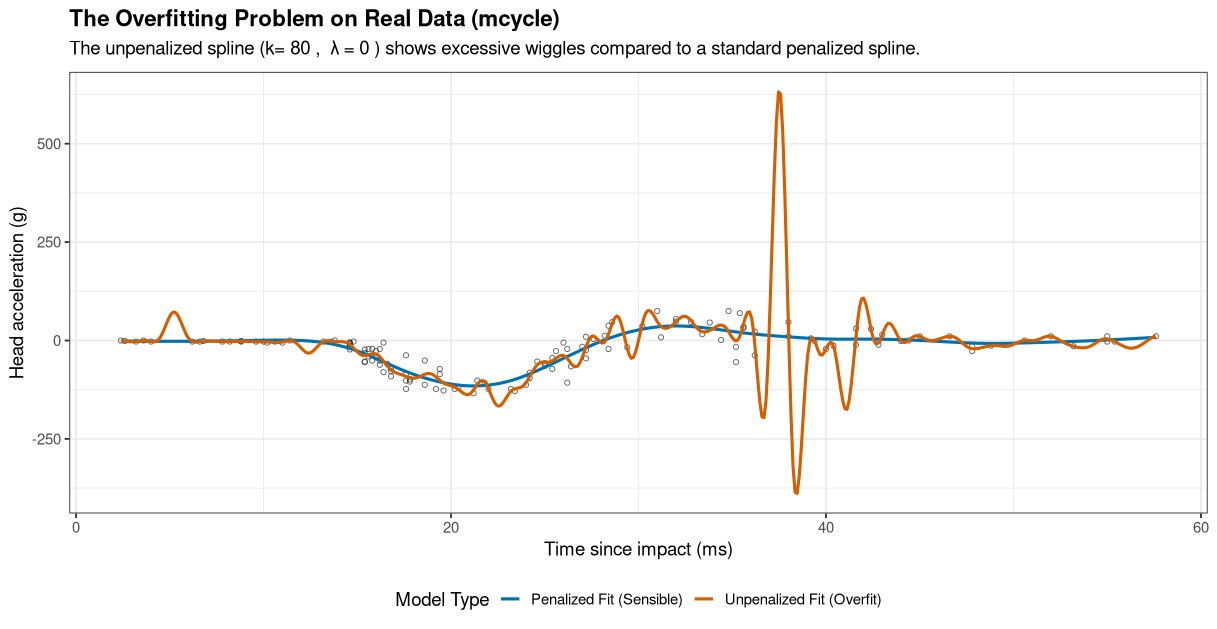
\includegraphics[width=\linewidth]{overfit.png}
  \caption{Overfitted spline}
  \label{fig:enter-label}
 \end{figure}
\subsection{2.3 Penalized Splines – A Principled Approach to Smoothness}
The  framework of penalized splines offers an elegant resolution to the twin problems of knot selection and overfitting. The core idea is to begin with a basis that is rich enough to represent complex functions—typically involving a generous number of knots that are often, though not necessarily, evenly spaced—and then to introduce a penalty term into the estimation criterion that explicitly discourages excessive "wiggliness" or complexity in the fitted function. The fitting process then automatically balances fidelity to the data against the smoothness imposed by this penalty.

The coefficients $\boldsymbol{\beta}$ of the basis functions are determined by minimizing a \textbf{penalized least squares objective function}:
\
This objective function has two main components:
\begin{enumerate}
 \item $||\mathbf{y} - \mathbf{X}\boldsymbol{\beta}||^2$: This is the standard sum of squared errors (SSE), measuring the goodness-of-fit of the model to the observed data $\mathbf{y}$. Minimizing this term alone would lead to an unpenalized fit, prone to overfitting if the basis $\mathbf{X}$ is rich.
 \item $\lambda \boldsymbol{\beta}^T \mathbf{S} \boldsymbol{\beta}$: This is the \textbf{penalty term} that quantifies the "wiggliness" of the function represented by $\boldsymbol{\beta}$.
 \begin{itemize}
  \item $\lambda \ge 0$ is the \textbf{smoothing parameter}. It is a crucial tuning parameter that controls the trade-off between goodness-of-fit and smoothness.
  \begin{itemize}
\item If $\lambda = 0$, there is no penalty, and the objective reduces to ordinary least squares. If the basis is rich, this can lead to overfitting, where the spline may interpolate the data.[10]
\item As $\lambda \rightarrow \infty$, the penalty term dominates the objective function. To minimize the overall expression, the model is forced to make $\boldsymbol{\beta}^T \mathbf{S} \boldsymbol{\beta}$ very small. This results in a very smooth function. For instance, with a typical second-derivative penalty, the fitted function will approach a straight line (the smoothest possible function in that context).
\item An appropriate, finite, positive value of $\lambda$ achieves a balance, producing a smooth function that captures the underlying trend in the data without fitting the noise. The selection of this optimal $\lambda$ is a key aspect of penalized spline methodology.
  \end{itemize}
  \item $\mathbf{S}$ is the \textbf{penalty matrix}. This $K \times K$ symmetric, positive semi-definite matrix defines precisely what constitutes "wiggliness" in terms of the basis coefficients $\boldsymbol{\beta}$. The structure of $\mathbf{S}$ depends on the chosen basis functions and the type of penalty applied (e.g., penalties based on integrated squared derivatives of $f(x)$ or penalties based on finite differences of the coefficients $\beta_k$). This will be explored in detail in Part 3.
 \end{itemize}
\end{enumerate}
A significant advantage of the penalized spline approach is that the \textbf{choice of knots becomes far less critical} than in classical regression splines. As long as a sufficiently large number of knots are used to span the range of the data and allow for potential complexity, their exact placement is not a primary concern. The smoothness of the resulting function is primarily controlled by the smoothing parameter $\lambda$, not by meticulous knot selection. For instance, a common strategy is to use a number of knots proportional to $\min(n/4, 40)$, often placed at quantiles of the predictor or simply evenly spaced. This "rich basis then constrain" philosophy is a general theme in modern statistical modeling: start with a model class flexible enough to capture complex signals and then use regularization to select a desirable solution from this class.

The penalty term $\lambda \boldsymbol{\beta}^T \mathbf{S} \boldsymbol{\beta}$ can be viewed as a form of shrinkage on the coefficients $\boldsymbol{\beta}$, analogous to ridge regression. However, unlike standard ridge regression where the penalty is $\lambda ||\boldsymbol{\beta}||_2^2 = \lambda \boldsymbol{\beta}^T \mathbf{I} \boldsymbol{\beta}$ (shrinking all coefficients uniformly towards zero), the penalty matrix $\mathbf{S}$ in penalized splines imposes a structured shrinkage. It specifically penalizes combinations of coefficients that lead to functions deemed too "wiggly" according to the definition embodied in $\mathbf{S}$.

\begin{figure}
 \centering
 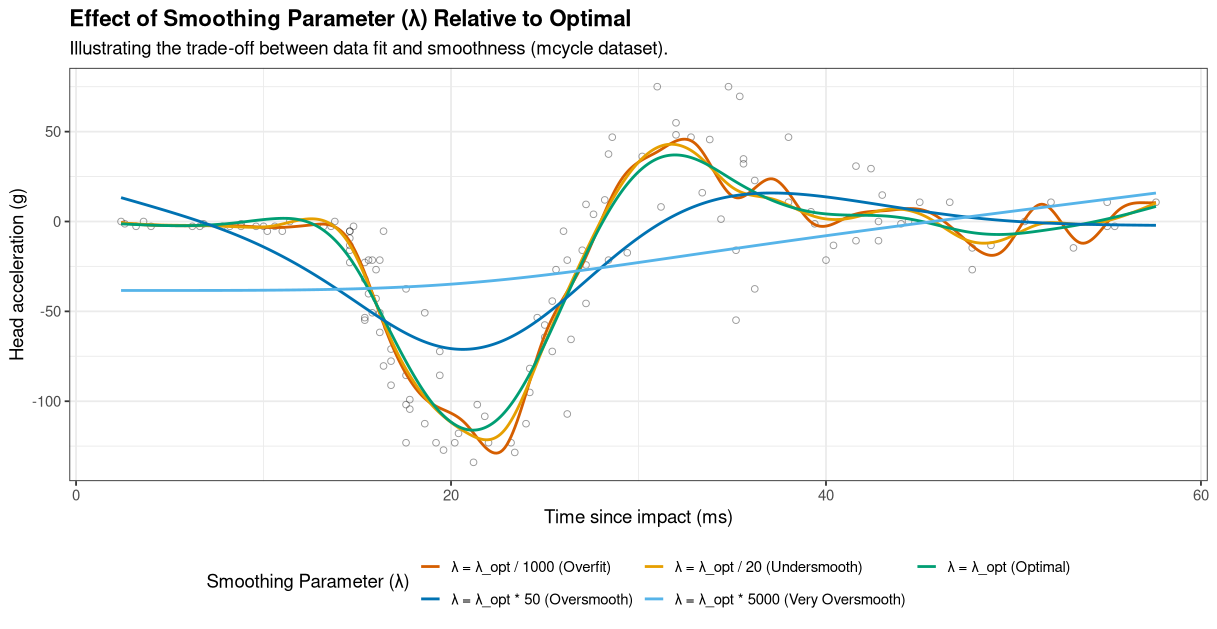
\includegraphics[width=\linewidth]{optimal_over_under.png}
 \caption{Visualisation of different choices of $\lambda$}
 \label{fig:enter-label}
\end{figure}

\newpage
\section{ Penalized Spline Components}
Having established the foundational problem and the conceptual solution offered by penalized splines, this section provides a more detailed mathematical examination of the core components: the basis expansion used to represent the smooth function, the construction and interpretation of the wiggliness penalty, the derivation of the penalized least squares solution, and the concept of effective degrees of freedom which quantifies model complexity.

\subsection{3.1 The Basis Expansion and Model Matrix $\mathbf{X}$}
The first step in constructing a penalized spline is to define a set of basis functions, $b_k(x)$, which are combined linearly to approximate the unknown smooth function $f(x)$. The choice of basis functions and their number, $K$, determines the flexibility of the function space within which we are searching for our estimate.

\paragraph{Mathematical Formulation}
The smooth function $f(x)$ is approximated by a linear combination of $K$ basis functions:
\[ f(x) = \sum_{k=1}^{K} \beta_k b_k(x) \]
Here, $b_k(x)$ is the $k$-th basis function, which is a known function of the covariate $x$, and $\beta_k$ is the corresponding coefficient that needs to be estimated from the data. The number of basis functions, $K$, is typically chosen to be sufficiently large to ensure that the basis is flexible enough to capture potentially complex patterns in the data, without being so excessively large as to create undue computational burden. In the penalized spline framework, the exact value of $K$ is less critical than in unpenalized regression splines, as the penalty term will control the effective smoothness.

\paragraph{Commonly Used Basis Functions}
Several types of basis functions are commonly employed in penalized spline models:
\begin{itemize}
 \item \textbf{B-splines:} B-splines are perhaps the most widely used basis functions for penalized splines, particularly for P-splines (discussed in Part 4). They are piecewise polynomial functions of a specified degree (e.g., cubic B-splines, which are piecewise cubic polynomials, are common). A key property of B-splines is their \textit{local support}: each basis function $b_k(x)$ is non-zero only over a limited range of $x$, typically spanning a few knot intervals. This local support leads to banded (sparse) model and penalty matrices, which is computationally advantageous, especially for large $K$. Visualizations of B-spline basis functions often show characteristic "bell-shaped" curves that overlap with their neighbors.

 \item \textbf{Truncated Power Series Basis:} Another way to represent splines is using a truncated power series basis. For a spline of degree $d$ with $M_{knots}$ interior knots $\kappa_1, \dots, \kappa_{M_{knots}}$, this basis consists of the polynomials $1, x, x^2, \dots, x^d$ and the truncated power functions $(x-\kappa_j)_+^d$ for $j=1, \dots, M_{knots}$. The function $(u)_+$ is defined as $u$ if $u > 0$ and $0$ otherwise. While conceptually simple, truncated power series bases can lead to severe numerical instability (ill-conditioning) when $K$ is large, due to high correlation between basis functions. B-splines are generally preferred for their superior numerical properties.

 \item Other bases, such as those derived from the eigenfunctions of differential operators (as in Thin Plate Regression Splines, see Section 4.2), are also used.
\end{itemize}
The choice of basis functions represents a trade-off between numerical stability, computational efficiency for constructing the basis and penalty matrices, and the ease with which certain types of penalties can be imposed.

\paragraph{Constructing the Model Matrix $\mathbf{X}$}
Given $n$ observations $(x_i, y_i)$, $i=1, \dots, n$, the vector of evaluated smooth function values $\mathbf{f} = [f(x_1), f(x_2), \dots, f(x_n)]^T$ can be expressed in matrix form as:
\[ \mathbf{f} = \mathbf{X}\boldsymbol{\beta} \]
where $\boldsymbol{\beta} = [\beta_1, \beta_2, \dots, \beta_K]^T$ is the $K \times 1$ vector of basis coefficients. The $n \times K$ matrix $\mathbf{X}$ is known as the \textbf{model matrix} (or design matrix). Each element $X_{ik}$ of this matrix is the value of the $k$-th basis function $b_k(x)$ evaluated at the $i$-th covariate value $x_i$:
\[ X_{ik} = b_k(x_i) \]
Thus, the $i$-th row of $\mathbf{X}$ is $[b_1(x_i), b_2(x_i), \dots, b_K(x_i)]$, and the $k$-th column is $[b_k(x_1), b_k(x_2), \dots, b_k(x_n)]^T$. The construction of this matrix is a standard procedure in software packages that implement splines; for example, the `splines2` package in R provides functions like `bSpline()` to generate B-spline basis matrices.

The use of a basis expansion effectively transforms the non-parametric problem of estimating an unknown function $f(x)$ into a parametric problem of estimating the coefficients $\boldsymbol{\beta}$, albeit often in a high-dimensional parameter space. This transformation is fundamental, as it allows the application of familiar (penalized) least squares or likelihood-based estimation techniques. The structure of $\mathbf{X}$ (e.g., its sparsity, conditioning) is directly influenced by the choice of basis functions and knot locations, which in turn affects computational efficiency and the numerical stability of the estimation process.

\subsection{3.2 The Wiggliness Penalty: $\lambda \boldsymbol{\beta}^T \mathbf{S} \boldsymbol{\beta}$}
The wiggliness penalty, $\lambda \boldsymbol{\beta}^T \mathbf{S} \boldsymbol{\beta}$, is the component of the penalized least squares objective that controls the smoothness of the fitted function. It quantifies the "roughness" or "complexity" of the function $f(x) = \sum \beta_k b_k(x)$ in terms of its coefficients $\boldsymbol{\beta}$.

\paragraph{Derivation from Integrated Squared Derivatives}
A classical approach to defining the wiggliness of a function $f(x)$ is to measure the energy associated with its derivatives. Commonly, the integral of the squared $m$-th derivative is used:
\[ \text{Penalty Functional} = \int [f^{(m)}(x)]^2 dx \]
For instance, if $m=2$, the penalty is $\int [f''(x)]^2 dx$, which penalizes functions with high curvature (rapidly changing slope), as in the physical analogy of the draftsman's spline.

To express this functional in terms of the basis coefficients $\boldsymbol{\beta}$, we substitute $f(x) = \sum_{k=1}^{K} \beta_k b_k(x)$. The $m$-th derivative is $f^{(m)}(x) = \sum_{k=1}^{K} \beta_k b_k^{(m)}(x)$. Let $\mathbf{b}^{(m)}(x)$ be the $K \times 1$ vector with elements $b_k^{(m)}(x)$. Then $f^{(m)}(x) = \boldsymbol{\beta}^T \mathbf{b}^{(m)}(x) = (\mathbf{b}^{(m)}(x))^T \boldsymbol{\beta}$.
The squared $m$-th derivative is $[f^{(m)}(x)]^2 = (\boldsymbol{\beta}^T \mathbf{b}^{(m)}(x)) ((\mathbf{b}^{(m)}(x))^T \boldsymbol{\beta}) = \boldsymbol{\beta}^T \left( \mathbf{b}^{(m)}(x) (\mathbf{b}^{(m)}(x))^T \right) \boldsymbol{\beta}$.
Integrating this expression yields:
\[ \int [f^{(m)}(x)]^2 dx = \boldsymbol{\beta}^T \left( \int \mathbf{b}^{(m)}(x) (\mathbf{b}^{(m)}(x))^T dx \right) \boldsymbol{\beta} \]
Thus, the penalty matrix $\mathbf{S}$ is a $K \times K$ matrix whose elements are given by:
\
This matrix $\mathbf{S}$ is symmetric and positive semi-definite. The penalty term becomes $\boldsymbol{\beta}^T \mathbf{S} \boldsymbol{\beta}$. For example, if $m=2$, $S_{jk} = \int b_j''(x) b_k''(x) dx$.[21]

\paragraph{P-spline Difference Penalties}
dAn alternative and computationally convenient approach, popularized by Eilers and Marx (1996) for P-splines, is to define the penalty based on finite differences of adjacent B-spline coefficients. This approximates the integrated derivative penalty but is often simpler to construct.
The rationale is that if the function is smooth, its B-spline coefficients should also form a smooth sequence. Large differences between adjacent coefficients imply rapid changes and thus "wiggliness."
Let $\Delta^m \beta_k$ denote the $m$-th order difference of the coefficients.
\begin{itemize}
 \item First-order difference ($m=1$): $\Delta \beta_k = \beta_k - \beta_{k-1}$ (penalizes jumps in coefficient values).
 \item Second-order difference ($m=2$): $\Delta^2 \beta_k = \Delta(\Delta \beta_k) = (\beta_k - \beta_{k-1}) - (\beta_{k-1} - \beta_{k-2}) = \beta_k - 2\beta_{k-1} + \beta_{k-2}$ (penalizes changes in the slope of the coefficient sequence, i.e., curvature).
\end{itemize}
The penalty is then the sum of squares of these differences: $\sum_{k} (\Delta^m \beta_k)^2$.
This sum can be expressed in matrix form. Let $\mathbf{D}_m$ be a differencing matrix of appropriate dimensions such that the vector of $m$-th differences is $\mathbf{D}_m \boldsymbol{\beta}$. Then the penalty is $(\mathbf{D}_m \boldsymbol{\beta})^T (\mathbf{D}_m \boldsymbol{\beta}) = \boldsymbol{\beta}^T \mathbf{D}_m^T \mathbf{D}_m \boldsymbol{\beta}$.
In this case, the penalty matrix is $\mathbf{S} = \mathbf{D}_m^T \mathbf{D}_m$.[17, 23]

For example, with $K$ coefficients:
\begin{itemize}
 \item For $m=1$, $\mathbf{D}_1$ is a $(K-1) \times K$ matrix:
 \
 \item For $m=2$, $\mathbf{D}_2$ is a $(K-2) \times K$ matrix:
 \
 \item For $m=3$, $\mathbf{D}_3$ is a $(K-3) \times K$ matrix:
 \
\end{itemize}
The choice of the order $m$ for the penalty reflects an implicit assumption about the nature of the function's smoothness. A second-order penalty ($m=2$) is very common, as it penalizes deviations from local linearity in the function (or its coefficients) and leads to visually smooth curves. The sparsity of $\mathbf{D}_m$ (it is a banded matrix) means that $\mathbf{S}=\mathbf{D}_m^T\mathbf{D}_m$ is also banded and sparse, which is computationally very efficient.

\paragraph{The Smoothing Parameter $\lambda$}
The scalar $\lambda \ge 0$ multiplies the entire penalty term $\boldsymbol{\beta}^T \mathbf{S} \boldsymbol{\beta}$. It governs the strength of the penalty and thus controls the trade-off between fitting the data closely and maintaining smoothness. A larger $\lambda$ imposes a heavier penalty on wiggliness, leading to a smoother function, while a smaller $\lambda$ allows the function to be more flexible and fit the data more closely. The selection of $\lambda$ is a critical aspect of penalized spline modeling and will be discussed further in Part 5.

The penalty term, by adding a regularization constraint, transforms what could be an ill-posed problem (fitting an overly flexible model to noisy data) into a well-posed one, ensuring a unique and stable solution.

\subsection{3.3 The Penalized Least Squares Solution $\hat{\boldsymbol{\beta}}$ and Influence Matrix $\mathbf{A}$}
The coefficients $\hat{\boldsymbol{\beta}}$ for the penalized spline are found by minimizing the penalized least squares objective function:
\
This is a quadratic function of $\boldsymbol{\beta}$, and its minimum can be found by setting its derivative with respect to $\boldsymbol{\beta}$ to zero.

\paragraph{Derivation of $\hat{\boldsymbol{\beta}}$}
The objective function can be expanded as:
\
\
Since $\mathbf{y}^T\mathbf{X}\boldsymbol{\beta}$ is a scalar, it is equal to its transpose $\boldsymbol{\beta}^T\mathbf{X}^T\mathbf{y}$. Assuming $\mathbf{S}$ is symmetric (which is standard for penalty matrices derived from squared derivatives or difference operators), we have:
\
To find the minimum, we differentiate $L(\boldsymbol{\beta})$ with respect to $\boldsymbol{\beta}$ and set the result to zero:
\
Setting this derivative to zero to find the optimal $\hat{\boldsymbol{\beta}}$:
\
Dividing by 2 and rearranging terms:
\
Assuming the matrix $(\mathbf{X}^T\mathbf{X} + \lambda\mathbf{S})$ is invertible (which is generally true if $\lambda > 0$ and $\mathbf{S}$ penalizes all functions not in the null space of $\mathbf{X}$), the solution for the penalized least squares coefficients is:
\
This solution is analogous to the ridge regression estimator, where $\mathbf{S}$ takes the place of the identity matrix $\mathbf{I}$ in the ridge penalty $\lambda \boldsymbol{\beta}^T\mathbf{I}\boldsymbol{\beta}$. The term $\lambda\mathbf{S}$ regularizes the problem, ensuring a unique solution even if $\mathbf{X}^T\mathbf{X}$ is singular or ill-conditioned, which can occur if $K$ is large or basis functions are highly collinear.

\paragraph{Fitted Values and the Influence Matrix $\mathbf{A}$}
The vector of fitted values, $\hat{\mathbf{y}}$, is obtained by applying the estimated coefficients to the model matrix:
\
This expression shows that the fitted values are a linear transformation of the observed responses $\mathbf{y}$. We can write this as:
\[ \hat{\mathbf{y}} = \mathbf{A}\mathbf{y} \]
where the $n \times n$ matrix
\
is called the \textbf{influence matrix} or \textbf{hat matrix} for the penalized spline smoother. Each element $A_{ij}$ represents the influence of the $j$-th observation $y_j$ on the $i$-th fitted value $\hat{y}_i$. The diagonal elements $A_{ii}$ are known as the leverage values, indicating how much influence each observation $y_i$ has on its own fitted value $\hat{y}_i$.[29, 30]

The influence matrix $\mathbf{A}$ is symmetric if $\mathbf{S}$ is symmetric. However, unlike the hat matrix in ordinary unpenalized least squares (where $\lambda=0$ and $\mathbf{S}=\mathbf{0}$, making $\mathbf{A} = \mathbf{X}(\mathbf{X}^T\mathbf{X})^{-1}\mathbf{X}^T$), the influence matrix for penalized splines with $\lambda > 0$ is generally \textit{not} idempotent (i.e., $\mathbf{A}\mathbf{A} \neq \mathbf{A}$). It becomes idempotent if $\lambda=0$ and $\mathbf{X}^T\mathbf{X}$ is invertible. The influence matrix plays a critical role in diagnostics, such as calculating residuals ($\mathbf{e} = (\mathbf{I}-\mathbf{A})\mathbf{y}$), and in the development of criteria for selecting the smoothing parameter $\lambda$, such as Generalized Cross-Validation (GCV).

\subsection{3.4 Effective Degrees of Freedom (EDF)}
In ordinary linear regression, the degrees of freedom consumed by the model is simply the number of estimated parameters (the rank of $\mathbf{X}$). For penalized models like penalized splines, the parameters $\boldsymbol{\beta}$ are not estimated freely; their values are constrained or "shrunk" by the penalty term. The \textbf{Effective Degrees of Freedom (EDF)} provides a measure of the model's complexity or flexibility that accounts for this shrinkage.

\paragraph{Definition and Formula}
The EDF for a penalized spline smoother is defined as the trace of the influence matrix $\mathbf{A}$:
\
Using the cyclic property of the trace, $\text{tr}(\mathbf{B}\mathbf{C}) = \text{tr}(\mathbf{C}\mathbf{B})$. The EDF is generally not an integer.

\paragraph{Interpretation}
The EDF quantifies the effective number of parameters being estimated by the model:
\begin{itemize}
 \item If $\lambda = 0$ (no penalty), and assuming $\mathbf{X}^T\mathbf{X}$ is invertible, then $\mathbf{A} = \mathbf{X}(\mathbf{X}^T\mathbf{X})^{-1}\mathbf{X}^T$. In this case, $EDF = \text{tr}(\mathbf{X}(\mathbf{X}^T\mathbf{X})^{-1}\mathbf{X}^T) = \text{tr}((\mathbf{X}^T\mathbf{X})^{-1}\mathbf{X}^T\mathbf{X}) = \text{tr}(\mathbf{I}_K) = K$, which is the number of basis functions (parameters).
 \item As $\lambda \rightarrow \infty$, the penalty term $\lambda \boldsymbol{\beta}^T \mathbf{S} \boldsymbol{\beta}$ dominates the objective function. The model forces $\boldsymbol{\beta}^T \mathbf{S} \boldsymbol{\beta}$ to be minimal. The fitted function $f(x)$ becomes a function in the null space of the penalty $\mathbf{S}$. For a typical $m$-th order derivative or difference penalty, this null space consists of polynomials of degree $m-1$. For example, with a second-derivative penalty ($m=2$), the null space is spanned by a constant and a linear term, so $EDF \rightarrow 2$. If $m=1$, $EDF \rightarrow 1$ (a constant function).
 \item For finite, positive values of $\lambda$, the EDF will be between the dimension of the null space of $\mathbf{S}$ and $K$. Specifically, if the null space of $\mathbf{S}$ has dimension $M_0$ (e.g., $M_0=m$ for an $m$-th order difference penalty), then $M_0 \le EDF \le K$.
\end{itemize}

A more intuitive understanding of EDF can be gained through a reparameterization where the model matrix is orthogonal and the penalty matrix is diagonal. Let $\mathbf{X} = \mathbf{Q}\mathbf{U}$ and $\mathbf{R}^{-T}\mathbf{S}\mathbf{R}^{-1} = \mathbf{U\Lambda U}^T$ from a transformation involving QR decomposition and eigen-decomposition. In this "natural" parameterization, the $j$-th penalized coefficient $\hat{\alpha}_j$ is related to its unpenalized counterpart $\tilde{\alpha}_j$ by $\hat{\alpha}_j = \tilde{\alpha}_j / (1 + \lambda \Lambda_{jj})$, where $\Lambda_{jj}$ are the eigenvalues of the transformed penalty matrix. The term $1 / (1 + \lambda \Lambda_{jj})$ is a shrinkage factor for the $j$-th "natural" parameter of the model. The EDF is then the sum of these shrinkage factors:
\
This formulation clearly shows that EDF is the sum of how much each underlying parameter is allowed to contribute to the fit, with each contribution scaled by the penalty.

The EDF is a crucial concept because it provides a measure of model complexity that is essential for model selection criteria like AIC (Akaike Information Criterion), where $AIC = -2 \log(\text{Likelihood}) + 2 \times EDF$, and for the GCV score denominator. Unlike the number of basis functions $K$, the EDF reflects the actual flexibility of the fitted smooth, which changes with $\lambda$. Notably, for a fixed $\lambda$, the EDF depends on $\mathbf{X}$ and $\mathbf{S}$ but not on the response data $\mathbf{y}$, making it an intrinsic property of the smoother's structure for that $\lambda$.

\begin{figure}
 \centering
 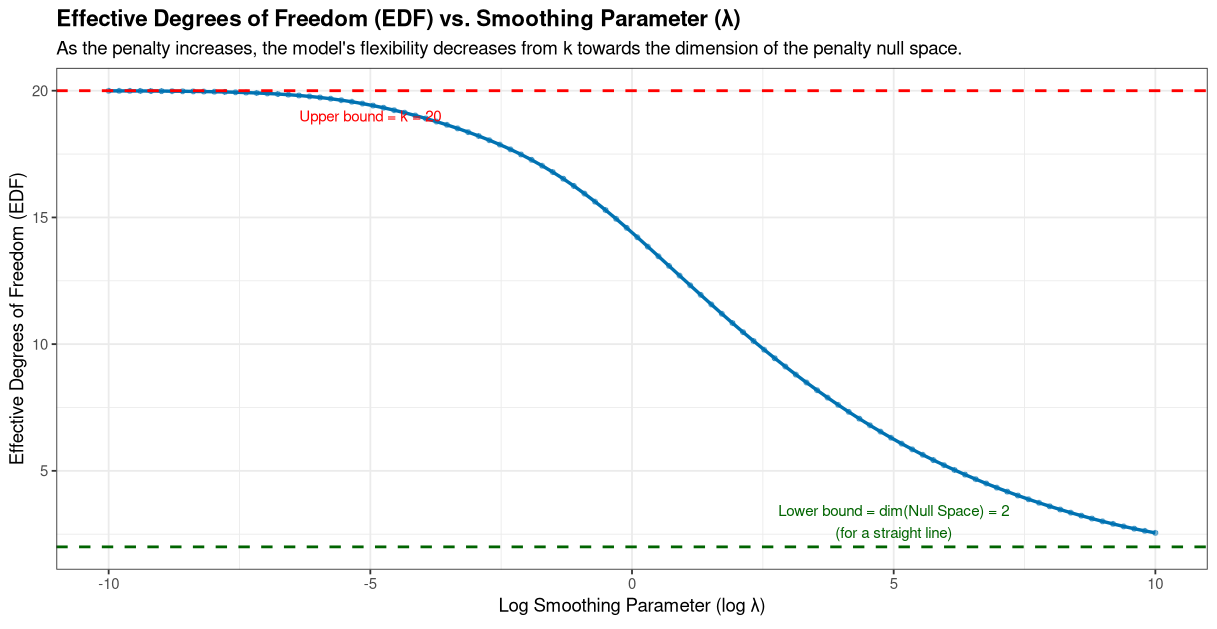
\includegraphics[width=1\linewidth]{edg_viz.png}
 \caption{EDF relationship with increase lambda}
 \label{fig:enter-label}
\end{figure}

\newpage
\section{Comparison of Key Spline Bases}
This section provides a detailed comparison of three prominent spline bases: P-splines, Thin Plate Regression Splines, and Adaptive Smoothers.

\begin{figure}
 \centering
 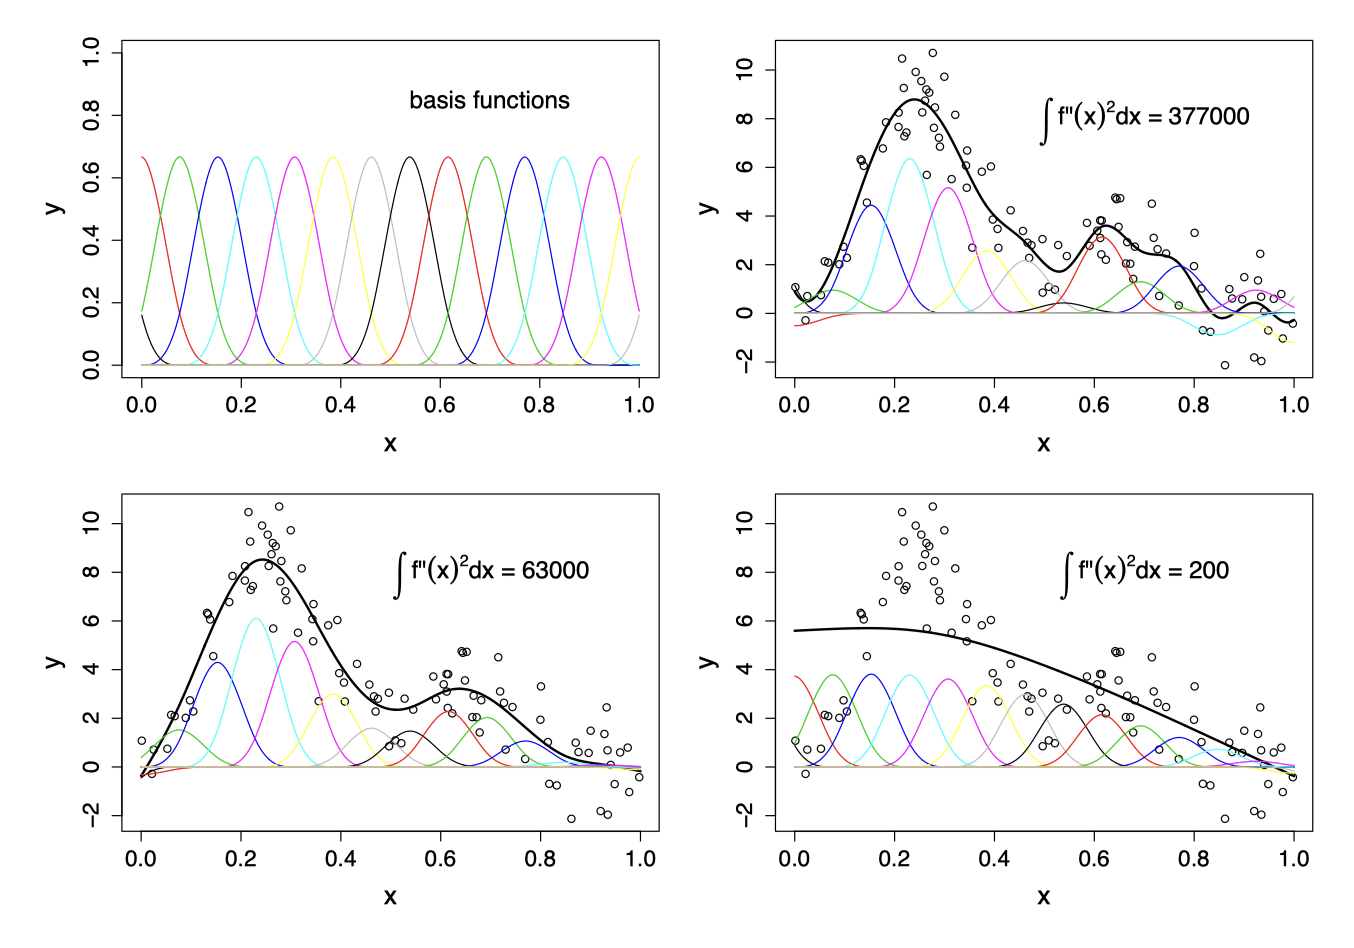
\includegraphics[width=\linewidth]{basis-penalty-illustration.png}
 \caption{Basis Penalty Illustration based on Wood, Basis Penalty Smoothers}
 \label{fig:enter-label}
\end{figure}
\subsection{4.1 P-Splines (`bs="ps"`)}
P-splines, introduced by Eilers and Marx (1996), represent a practical and computationally efficient approach to penalized spline smoothing. They combine a B-spline basis with a discrete penalty based on finite differences of adjacent B-spline coefficients.

\paragraph{Basis: B-splines with Evenly Spaced Knots}
P-splines employ B-spline basis functions $b_k(x)$. As detailed in Section 3.1, B-splines are piecewise polynomials of a specified degree (cubic B-splines are a common choice) and possess local support, meaning each $b_k(x)$ is non-zero only over a few adjacent knot intervals.
A defining characteristic of P-splines is the use of a relatively large number of knots that are \textbf{evenly spaced} over the domain of the covariate $x$. This deliberate choice simplifies the construction of the penalty matrix and, more importantly, makes the precise number and location of knots non-critical for the quality of the fit, as the effective smoothness is primarily controlled by the smoothing parameter $\lambda$ associated with the penalty. The number of basis functions, $K$, is typically chosen to be moderately large (e.g., $K=10$ to $K=40$) to ensure sufficient flexibility to capture complex patterns if present. 

\paragraph{Penalty: Discrete Differences of Adjacent Coefficients}
The penalty in P-splines targets the differences between coefficients $\beta_k$ of adjacent B-spline basis functions. This is based on the intuition that a smooth function should have smoothly varying B-spline coefficients.
For an $m$-th order difference penalty, the penalty term is $\lambda \sum_{k} (\Delta^m \beta_k)^2$, where $\Delta^m \beta_k$ is the $m$-th order difference.
\begin{itemize}
 \item $\Delta \beta_k = \beta_k - \beta_{k-1}$ (first-order difference)
 \item $\Delta^2 \beta_k = \beta_k - 2\beta_{k-1} + \beta_{k-2}$ (second-order difference, using appropriate indexing for $\beta_k, \beta_{k-1}, \beta_{k-2}$).[17, 25]
 \item $\Delta^3 \beta_k = \beta_k - 3\beta_{k-1} + 3\beta_{k-2} - \beta_{k-3}$ (third-order difference).
\end{itemize}
The penalty matrix takes the form $\mathbf{S} = \mathbf{D}_m^T \mathbf{D}_m$, where $\mathbf{D}_m$ is the matrix operator that computes the $m$-th order differences.
For example, if $K=5$ coefficients $\boldsymbol{\beta} = [\beta_1, \beta_2, \beta_3, \beta_4, \beta_5]^T$:
\begin{itemize}
 \item The first-order difference matrix $\mathbf{D}_1$ (of size $(K-1) \times K$) would be:
 \
 yielding $\mathbf{D}_1 \boldsymbol{\beta} = [\beta_2-\beta_1, \beta_3-\beta_2, \beta_4-\beta_3, \beta_5-\beta_4]^T$.

 \item The second-order difference matrix $\mathbf{D}_2$ (of size $(K-2) \times K$) would be:
 \
 yielding $\mathbf{D}_2 \boldsymbol{\beta} = [\beta_1-2\beta_2+\beta_3, \beta_2-2\beta_3+\beta_4, \beta_3-2\beta_4+\beta_5]^T$. (Note: The exact form of differences, e.g., forward, backward, or centered, can vary, but the principle of penalizing $m$-th order differences remains. The matrix shown corresponds to centered differences for the interior coefficients if we imagine the sequence $\beta_k$).

 \item The third-order difference matrix $\mathbf{D}_3$ (of size $(K-3) \times K$) would be:
 \
 yielding $\mathbf{D}_3 \boldsymbol{\beta} = [-\beta_1+3\beta_2-3\beta_3+\beta_4, -\beta_2+3\beta_3-3\beta_4+\beta_5]^T$.
\end{itemize}
The matrix $\mathbf{D}_m$ is sparse (banded), and consequently, $\mathbf{S} = \mathbf{D}_m^T \mathbf{D}_m$ is also sparse (banded), which leads to significant computational efficiencies.[34]

\paragraph{Advantages and Characteristics}
P-splines offer several advantages:
\begin{itemize}
 \item \textbf{Computational Simplicity and Efficiency:} The use of B-splines with equally spaced knots and sparse difference penalty matrices makes P-splines easy to construct and computationally efficient, especially for large datasets.[34]
 \item \textbf{Intuitive Penalty:} The difference penalty is conceptually straightforward; it directly penalizes rapid changes in the sequence of B-spline coefficients.
 \item \textbf{Flexibility in Orders:} P-splines allow for flexible "mixing-and-matching" of the B-spline basis order (e.g., linear, quadratic, cubic B-splines) and the order of the difference penalty ($m$).[34] A common choice is cubic B-splines with a second or third-order difference penalty.
 \item \textbf{Good Performance:} They are often a "workhorse" for univariate smoothing in GAMs due to their good empirical performance and robustness.
 \item \textbf{Bayesian Connection:} The P-spline penalty has a direct Bayesian interpretation as imposing a Gaussian random walk prior on the B-spline coefficients. For instance, a second-order difference penalty corresponds to a second-order random walk prior, $ \beta_k | \beta_{k-1}, \beta_{k-2} \sim N(2\beta_{k-1} - \beta_{k-2}, \sigma_\beta^2) $, where $\sigma_\beta^2$ is related to $1/\lambda$. This connection facilitates Bayesian estimation using MCMC methods and the integration of P-splines into hierarchical Bayesian models.
\end{itemize}


\subsection{4.2 Thin Plate Regression Splines (`bs="tp"`): The Eigen-Based Approach}
Thin Plate Splines (TPS) are a class of smoothers that are optimal in the sense that they minimize a "bending energy" functional, generalizing the draftsman's physical spline to multiple dimensions. Full TPS involve a basis function for each data point, making them computationally intensive for large datasets ($O(n^3)$ complexity). Thin Plate \textit{Regression} Splines (TPRS), as developed by Wood (2003), address this by constructing an optimal, lower-rank approximate basis, thereby avoiding explicit knot selection and significantly reducing computational cost.

\paragraph{The Thin Plate Spline Penalty Functional}
The penalty for a thin plate spline measures its "wiggliness" by integrating squared $m$-th order partial derivatives over the domain of the covariates. For a function $f(\mathbf{x})$ of $d$ covariates, the general penalty functional is:
\[ J_{m,d}(f) = \sum_{\nu_1+\dots+\nu_d = m} \frac{m!}{\nu_1! \dots \nu_d!} \int \left( \frac{\partial^m f}{\partial x_1^{\nu_1} \dots \partial x_d^{\nu_d}} \right)^2 d\mathbf{x} \]
A common case is $m=2$. For $d=1$, this reduces to $\int (f''(x))^2 dx$. For $d=2$ (covariates $x_1, x_2$), the $m=2$ penalty is:
\[ J_{2,2}(f) = \iint \left\{ \left(\frac{\partial^2 f}{\partial x_1^2}\right)^2 + 2\left(\frac{\partial^2 f}{\partial x_1 \partial x_2}\right)^2 + \left(\frac{\partial^2 f}{\partial x_2^2}\right)^2 \right\} dx_1 dx_2 \]
This penalty is isotropic, meaning it penalizes curvature equally in all directions, which is appropriate when covariates are on comparable scales or when no specific directional preference for smoothness exists.

\paragraph{The Null Space of the Penalty}
The TPS penalty $J_{m,d}(f)$ is zero for any polynomial in $d$ variables of total degree less than $m$. These functions form the \textbf{null space} of the penalty and are not penalized by $\mathbf{S}$. For example, if $m=2$, the null space consists of linear functions (and constants), and its dimension is $M = \binom{m+d-1}{d} = \binom{d+1}{d} = d+1$. These $M$ polynomial basis functions must be included in the spline basis and are estimated without shrinkage by the penalty term.

\paragraph{Eigen-Decomposition and Optimal Basis Construction}
The core idea of TPRS is to find a low-rank basis that best approximates the full thin plate spline. This is achieved through an eigen-decomposition related to the penalty structure 
\begin{enumerate}
 \item \textbf{Full Penalty and Basis:} Conceptually, one starts with a basis and penalty structure corresponding to a full TPS (e.g., knots at all unique data locations). Let $\mathbf{S}_{full}$ be the penalty matrix associated with this full basis.
 \item \textbf{Eigen-decomposition:} The penalty matrix $\mathbf{S}_{full}$ (or a related matrix derived from it in the construction of TPRS, see Wood (2003) ) undergoes an eigen-decomposition: $\mathbf{S}_{full} = \mathbf{U \Lambda U}^T$. The columns of $\mathbf{U}$ are the eigenvectors, and $\mathbf{\Lambda}$ is a diagonal matrix of corresponding eigenvalues.
 \item \textbf{Identifying Unpenalized and Penalized Components:}
 \begin{itemize}
\item The $M$ eigenvectors corresponding to zero eigenvalues of $\mathbf{S}_{full}$ span the null space of the penalty (the unpenalized polynomials).
\item The eigenvectors corresponding to positive eigenvalues span the space of "wiggly" functions that are subject to penalization. The magnitude of an eigenvalue $\Lambda_{ii}$ reflects the degree of wiggliness associated with its corresponding eigenvector $\mathbf{u}_i$: smaller positive eigenvalues correspond to smoother functions (less penalty per unit norm of coefficients), while larger eigenvalues correspond to more wiggly functions.
 \end{itemize}
 \item \textbf{Optimal Truncation for Rank-$k$ Basis:} To construct a TPRS basis of a specified rank $k$ (where $k$ is typically much smaller than $n$):
\begin{itemize}
\item The $M$ basis functions spanning the null space are always included.
\item From the remaining eigenvectors (those with positive eigenvalues), the $k-M$ eigenvectors corresponding to the $k-M$ \textit{smallest positive} eigenvalues are selected. These represent the "smoothest" functions in the penalized space.[41, 45]
 \end{itemize}
 \item \textbf{Model and Penalty Matrices:} The model matrix $\mathbf{X}$ for the TPRS is formed using these $k$ selected basis functions ( $M$ null space functions and $k-M$ selected eigenvectors). The penalty matrix $\mathbf{S}$ for this TPRS basis becomes diagonal in this reparameterized representation, with entries corresponding to the $k-M$ selected positive eigenvalues and zeros for the $M$ null space components.
\end{enumerate}
This construction ensures that, for a given rank $k$, the TPRS basis is the best $k$-dimensional approximation to the full TPS in terms of minimizing the perturbation to the smoothing problem.[37]

\paragraph{Reparameterization and Simplified Penalty}
If the original spline coefficients are $\boldsymbol{\beta}$ and the coefficients for the eigenbasis are $\boldsymbol{\alpha}$ (such that $\boldsymbol{\beta} = \mathbf{U}\boldsymbol{\alpha}$), the penalty term $\lambda \boldsymbol{\beta}^T \mathbf{S}_{full} \boldsymbol{\beta}$ transforms to $\lambda \boldsymbol{\alpha}^T \mathbf{\Lambda} \boldsymbol{\alpha} = \lambda \sum_{i=1}^{K} \Lambda_{ii} \alpha_i^2$. The truncation step effectively sets $\alpha_i = 0$ for the components corresponding to the discarded eigenvectors (those with large eigenvalues, representing very wiggly functions). For the selected $k-M$ penalized components, the penalty is $\lambda \sum_{j=1}^{k-M} \Lambda_{j}^* \alpha_j^{*2}$, where $\Lambda_j^*$ are the smallest positive eigenvalues.

\paragraph{Advantages and Characteristics}
\begin{itemize}
 \item \textbf{Knot-free Definition:} TPRS entirely avoids the subjective and often problematic process of knot selection. The basis dimension $k$ is specified, but not knot locations.
 \item \textbf{Optimality:} The low-rank basis is chosen in a principled way to be an optimal approximation of the full thin plate spline, minimizing information loss for a given basis size.[37]
 \item \textbf{Multi-dimensional Smoothing:} TPRS are naturally defined for any number of covariates $d$ and are particularly well-suited for modeling interactions and smooth surfaces in multiple dimensions.
 \item \textbf{Isotropy:} The standard TPRS penalty is isotropic, treating all covariates (and directions in the covariate space) equally in terms of smoothing. This is an advantage when covariates are on similar scales and no prior knowledge suggests directional differences in smoothness.
\end{itemize}
The eigen-decomposition approach of TPRS is conceptually related to Principal Components Analysis (PCA). Just as PCA identifies principal components that capture the most variance, the eigen-decomposition here identifies basis functions (eigenfunctions of the penalty operator) that are ordered by their intrinsic smoothness (or wiggliness, as quantified by the eigenvalues). By selecting the smoothest of these, TPRS constructs a reduced-rank basis that retains the most important smooth features. TPRS are a default choice for multi-dimensional smoothing in `mgcv` due to these desirable properties.[38]

\subsection{4.3 Adaptive Smoothers (`bs="ad"`)}
Standard penalized splines assume that the optimal degree of smoothness is constant across the entire domain of the covariate(s). However, many real-world functions exhibit varying complexity: they might be very smooth (nearly linear) in some regions and highly variable or oscillatory in others. An adaptive smoother is designed for such situations by allowing the penalty strength, and thus the effective smoothness of the fit, to vary with the covariate values.

\paragraph{Intuition: The Smart Sander Analogy}
Imagine sanding a piece of wood that has some very rough patches and some nearly finished patches. Using a standard smoother (like a P-spline with a single $\lambda$) is analogous to using the same grit sandpaper across the entire piece. It might work reasonably well if the wood is uniformly rough, but it's a compromise. You would risk either oversanding the smooth parts (losing detail) or undersanding the rough parts (leaving them unfinished). An adaptive smoother is like a "smart sander" that automatically senses the local roughness of the wood and adjusts its grit size accordingly—using coarse grit on the rough patches and fine grit on the smooth ones.

\paragraph{Mechanism: Spatially Varying Penalty Weights}
The adaptive smoother in `mgcv` (`bs="ad"`) achieves this by modifying the standard P-spline penalty. A regular P-spline penalty is $\mathcal{P} = \lambda \sum_{k} (\Delta^m \beta_k)^2$. The adaptive version introduces spatially-varying weights, $\omega_k$:
\[ \mathcal{P}_a = \lambda \sum_{k} \omega_k (\Delta^m \beta_k)^2 \]
These weights $\omega_k > 0$ control the local penalty strength:
\begin{itemize}
 \item Where $\omega_k$ is \textbf{large}, the penalty is strong, forcing the function to be locally smooth.
 \item Where $\omega_k$ is \textbf{small}, the penalty is weak, allowing the function to be locally wiggly to capture rapid changes in the data.
\end{itemize}
In matrix form, the penalty is $\lambda \boldsymbol{\beta}^T \mathbf{D}_m^T \text{diag}(\boldsymbol{\omega}) \mathbf{D}_m \boldsymbol{\beta}$.

\paragraph{How are the Weights Determined?}
The key innovation is that the weights $\omega_k$ are not pre-specified but are themselves estimated from the data. They are modeled as a smooth function of their index $k$ (which corresponds to location along the covariate $x$). To ensure the weights vary smoothly and remain positive, their logarithm is typically modeled using another spline (a "meta-spline"):
\[ \log(\omega_k) = \sum_{j=1}^{K_{\omega}} \gamma_j b_{\omega,j}(k) \quad \text{or in matrix form} \quad \log(\boldsymbol{\omega}) = \mathbf{B}_{\omega}\boldsymbol{\gamma} \]
Here, $\mathbf{B}_{\omega}$ is a basis matrix (e.g., a B-spline basis) for the log-weights, and $\boldsymbol{\gamma}$ are the coefficients of this meta-spline. These coefficients $\boldsymbol{\gamma}$ effectively become additional smoothing parameters for the model. The model now has multiple smoothing parameters to estimate, which control how the main penalty varies.

The model is fitted using an iterative process that alternates between estimating the main function and estimating the penalty weights. This allows the smoother to "learn" where it needs to be more or less flexible. This hierarchical structure—a spline for the function whose penalty is controlled by another spline—is why it can be thought of as a GAM within a GAM penalty.

While powerful, adaptive smoothers are more complex and have more parameters to estimate. They generally require more data than standard smoothers to reliably estimate the varying smoothness structure and are computationally more intensive. They are particularly useful when visual inspection of the data or prior knowledge suggests that the assumption of constant smoothness is likely to be violated.
\begin{figure}
 \centering
 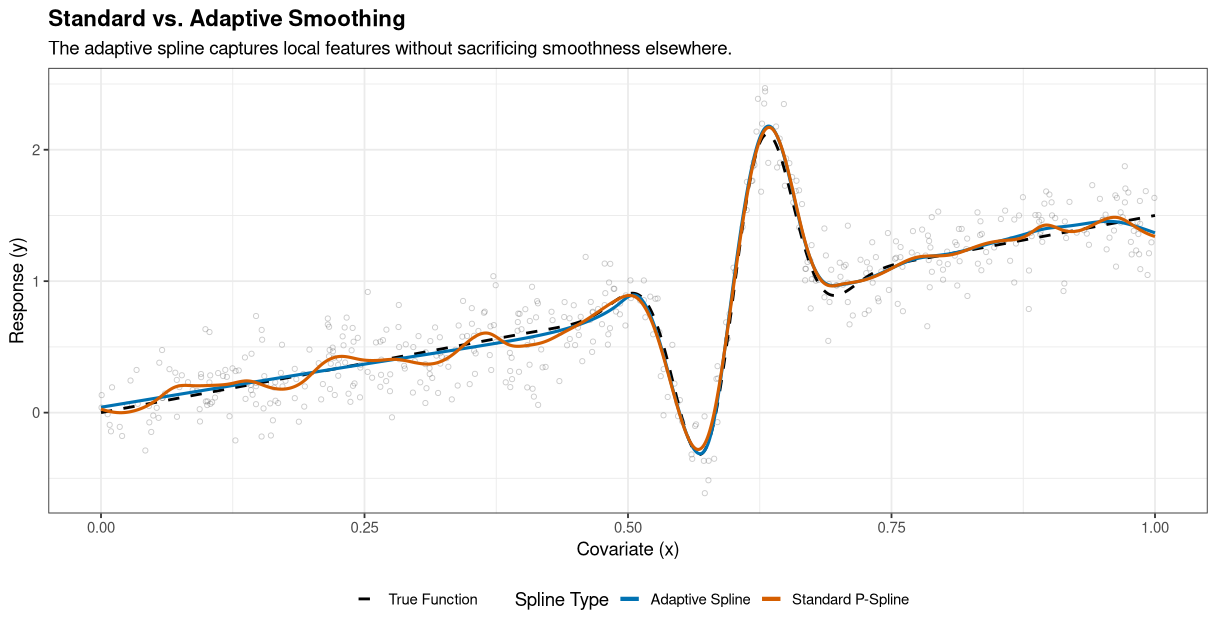
\includegraphics[width=1\linewidth]{adaptive_spline.png}
 \caption{Adaptive vs P-Spline}
\end{figure}

\vspace{1em}
\begin{table}[h!]
\centering
\caption{Comparison of Key Penalized Spline Bases in `mgcv`}
\label{tab:spline_comparison}
\begin{tabular}{@{}lllll@{}}
\toprule
\textbf{\texttt{mgcv} ID} & \textbf{Spline Type Name} & \textbf{Underlying Basis} & \textbf{Knot Strategy} & \textbf{Penalty Nature} \\
\midrule
`bs="ps"` & P-Spline & B-splines & Evenly spaced (many) & Discrete differences \\
& & (e.g., cubic) & User specifies $K$ & of coefficients \\
& & & & (e.g., $\sum (\Delta^2 \beta_k)^2$) \\
\addlinespace
`bs="tp"` & Thin Plate & Eigenfunctions of & Knot-free (implicit); & Integrated squared \\
& Regression Spline & TPS operator & User specifies basis rank $k$ & $m$-th derivatives \\
& & & &  \\
\addlinespace
`bs="ad"` & Adaptive P-Spline & B-splines for function; & Evenly spaced for & Weighted discrete \\
& & B-splines for penalty & underlying P-spline & differences of coeff. \\
& & weights & & $\sum \omega_k (\Delta^m \beta_k)^2$ \\
\bottomrule
\end{tabular}
\par
\vspace{0.5em}
\textit{Note:} $K$ is the number of basis functions. $\Delta^m \beta_k$ is the $m$-th order difference of coefficients. $\omega_k$ are spatially varying weights.
\end{table}

\newpage
\section{Penalized Likelihood and Bayesian Inference}
The framework of penalized splines, while often introduced from a perspective of optimizing a penalized goodness-of-fit criterion, possesses deep and illuminating connections to Bayesian statistical methodology. This section explores these connections, starting with the frequentist view of penalized likelihood and smoothing parameter selection via Generalized Cross-Validation (GCV), then bridging to the Bayesian interpretation where the penalty term is equivalent to a prior distribution. Finally, it details Empirical Bayes (REML/ML) and full Bayesian approaches for estimating smoothing parameters and conducting inference.

\subsection{5.1 The Frequentist View: Penalized Likelihood as Optimization}
From a frequentist perspective, the estimation of a penalized spline involves finding the vector of basis coefficients $\boldsymbol{\beta}$ that minimizes the penalized least squares objective function, as previously defined:
\
In this framework, the smoothing parameter $\lambda$ is typically treated as a fixed "tuning parameter" rather than a parameter to be estimated simultaneously with $\boldsymbol{\beta}$.[9] Its value must be determined externally, often by optimizing some criterion that estimates the model's out-of-sample prediction error.

\paragraph{Generalized Cross-Validation (GCV) for Smoothing Parameter Selection}
One of the most widely used methods for selecting $\lambda$ is Generalized Cross-Validation (GCV). GCV provides an efficient approximation to Leave-One-Out Cross-Validation (LOOCV) for linear smoothers, avoiding the computational burden of refitting the model $n$ times.

The intuition behind LOOCV is to estimate the prediction error by, for each observation $i$, fitting the model using all data points \textit{except} $(x_i, y_i)$, and then predicting $y_i$ with this model, denoted $\hat{f}_{(-i)}(x_i)$. The LOOCV error is the average squared prediction error: $CV(\lambda) = \frac{1}{n} \sum_{i=1}^n (y_i - \hat{f}_{(-i)}(x_i))^2$.
For linear smoothers where the fitted values are given by $\hat{\mathbf{y}} = \mathbf{A}(\lambda)\mathbf{y}$ (with $\mathbf{A}(\lambda) = \mathbf{X}(\mathbf{X}^T\mathbf{X} + \lambda\mathbf{S})^{-1}\mathbf{X}^T$ being the influence matrix), a remarkable result allows LOOCV to be calculated from a single model fit:
\[ CV(\lambda) = \frac{1}{n} \sum_{i=1}^n \left( \frac{y_i - \hat{y}_i(\lambda)}{1 - A_{ii}(\lambda)} \right)^2 \]
where $A_{ii}(\lambda)$ is the $i$-th diagonal element of the influence matrix $\mathbf{A}(\lambda)$.

The GCV score, $\mathcal{V}_g(\lambda)$, approximates $CV(\lambda)$ by replacing the individual leverage values $A_{ii}(\lambda)$ with their average, $\text{tr}(\mathbf{A}(\lambda))/n$:
\[ \mathcal{V}_g(\lambda) = \frac{1}{n} \sum_{i=1}^n \left( \frac{y_i - \hat{y}_i(\lambda)}{1 - \text{tr}(\mathbf{A}(\lambda))/n} \right)^2 \]
This can be rewritten in a more common form:
\[ \mathcal{V}_g(\lambda) = \frac{n ||\mathbf{y} - \mathbf{A}(\lambda)\mathbf{y}||^2}{[n - \text{tr}(\mathbf{A}(\lambda))]^2} \]
where $||\mathbf{y} - \mathbf{A}(\lambda)\mathbf{y}||^2$ is the residual sum of squares (RSS) for a given $\lambda$, and $\text{tr}(\mathbf{A}(\lambda))$ is the Effective Degrees of Freedom (EDF) of the model.  The smoothing parameter $\lambda$ is then chosen to minimize this $\mathcal{V}_g(\lambda)$ score. The denominator term $[n - \text{tr}(\mathbf{A}(\lambda))]^2$ penalizes model complexity; as $\text{tr}(\mathbf{A}(\lambda))$ (EDF) approaches $n$, the denominator becomes small, inflating the GCV score and thus disfavoring overly complex, interpolating fits.

The computational efficiency of GCV, requiring only one fit per candidate $\lambda$ to obtain $\mathbf{A}(\lambda)$, was instrumental in making automated smoothness selection practical for penalized splines and GAMs. While GCV is a powerful tool, it has been observed to sometimes select values of $\lambda$ that are too small, leading to undersmoothing, particularly with smaller sample sizes or when the true underlying function is very smooth.  This observation motivated the development of alternative estimation methods like REML and ML. Other criteria such as AIC, Mallows' $C_p$, or BIC can also be adapted for smoothing parameter selection, often involving the EDF in their penalty terms.

\subsection{5.2 The Bridge: The Penalty as a Prior}
A profound connection exists between the frequentist penalized likelihood approach and Bayesian inference. The penalized least squares objective function is mathematically equivalent to the negative log-posterior density of a specific Bayesian model. This equivalence provides a Bayesian interpretation for the penalty term: it corresponds to a prior distribution on the model coefficients $\boldsymbol{\beta}$.

\paragraph{Derivation of Equivalence to MAP Estimation}
We aim to show that minimizing $\mathcal{L}_{pen}(\boldsymbol{\beta}) = ||\mathbf{y} - \mathbf{X}\boldsymbol{\beta}||^2 + \lambda \boldsymbol{\beta}^T \mathbf{S} \boldsymbol{\beta}$ is equivalent to finding the Maximum A Posteriori (MAP) estimate of $\boldsymbol{\beta}$ under certain distributional assumptions.

The posterior probability of the coefficients $\boldsymbol{\beta}$, given the data $\mathbf{y}$, smoothing parameter $\lambda$, and error variance $\sigma^2$, is given by Bayes' theorem :
\[ P(\boldsymbol{\beta} | \mathbf{y}, \lambda, \sigma^2) \propto P(\mathbf{y} | \boldsymbol{\beta}, \sigma^2) P(\boldsymbol{\beta} | \lambda, \sigma^2) \]
where $P(\mathbf{y} | \boldsymbol{\beta}, \sigma^2)$ is the likelihood of the data given the coefficients, and $P(\boldsymbol{\beta} | \lambda, \sigma^2)$ is the prior distribution of the coefficients.

\begin{enumerate}
 \item \textbf{Likelihood $P(\mathbf{y} | \boldsymbol{\beta}, \sigma^2)$:}
 We assume that the errors $\epsilon_i = y_i - \mathbf{x}_i^T\boldsymbol{\beta}$ are independent and identically distributed Gaussian random variables with mean 0 and variance $\sigma^2$. Thus, $y_i | \mathbf{x}_i, \boldsymbol{\beta} \sim N(\mathbf{x}_i^T\boldsymbol{\beta}, \sigma^2)$. The likelihood for the entire dataset $\mathbf{y}$ is the product of individual likelihoods:
 \begin{align*}
 P(\mathbf{y} | \boldsymbol{\beta}, \sigma^2) &= \prod_{i=1}^n \frac{1}{\sqrt{2\pi\sigma^2}} \exp\left(-\frac{(y_i - \mathbf{x}_i^T\boldsymbol{\beta})^2}{2\sigma^2}\right) \\
 &= (2\pi\sigma^2)^{-n/2} \exp\left(-\frac{1}{2\sigma^2}\sum_{i=1}^n (y_i - \mathbf{x}_i^T\boldsymbol{\beta})^2\right) \\
 &= (2\pi\sigma^2)^{-n/2} \exp\left(-\frac{1}{2\sigma^2}||\mathbf{y} - \mathbf{X}\boldsymbol{\beta}||^2\right)
 \end{align*}
. 

 \item \textbf{Prior $P(\boldsymbol{\beta} | \lambda, \sigma^2)$:}
 We define a Gaussian prior distribution for the coefficients $\boldsymbol{\beta}$. The structure of this prior is chosen to correspond to the penalty term $\lambda \boldsymbol{\beta}^T \mathbf{S} \boldsymbol{\beta}$. A suitable prior is a (possibly improper if $\mathbf{S}$ is rank-deficient) multivariate Gaussian distribution with mean $\mathbf{0}$ and precision matrix $\frac{\lambda}{\sigma^2}\mathbf{S}$:
 \
 The normalization constant involving $|\frac{\lambda}{\sigma^2}\mathbf{S}|_+^{1/2}$ is omitted as it does not affect the mode of the posterior. This prior expresses a belief that smoother functions (those with smaller values of $\boldsymbol{\beta}^T\mathbf{S}\boldsymbol{\beta}$) are more probable, a priori.[61] The term $\lambda/\sigma^2$ indicates that the strength of this prior belief is scaled by the ratio of the penalty strength to the data variance.
\end{enumerate}

\paragraph{Log-Posterior and MAP Estimation}
The logarithm of the posterior distribution is:
\begin{align*}
 \log P(\boldsymbol{\beta} | \mathbf{y}, \lambda, \sigma^2) &\propto \log P(\mathbf{y} | \boldsymbol{\beta}, \sigma^2) + \log P(\boldsymbol{\beta} | \lambda, \sigma^2) \\
 &\propto -\frac{n}{2}\log(2\pi\sigma^2) - \frac{1}{2\sigma^2}||\mathbf{y} - \mathbf{X}\boldsymbol{\beta}||^2 - \frac{\lambda}{2\sigma^2}\boldsymbol{\beta}^T\mathbf{S}\boldsymbol{\beta}
\end{align*}
To find the MAP estimate, $\hat{\boldsymbol{\beta}}_{MAP}$, we maximize this log-posterior with respect to $\boldsymbol{\beta}$. This is equivalent to minimizing the negative of the terms involving $\boldsymbol{\beta}$:
\
Since $2\sigma^2$ is a positive constant (assuming $\sigma^2 > 0$), multiplying the objective by $2\sigma^2$ does not change the location of the minimum. This yields:
\
This is precisely the frequentist penalized least squares objective function.[58, 59, 60, 61, 62, 63, 64]

Therefore, the penalized least squares estimate $\hat{\boldsymbol{\beta}}$ is identical to the Bayesian MAP estimate under a Gaussian likelihood for the data and a specific Gaussian prior for the coefficients whose precision matrix is proportional to the penalty matrix $\mathbf{S}$. This establishes that the penalty term is not merely an ad-hoc device to control complexity but has a formal interpretation as encoding prior information favoring smoother functions. The smoothing parameter $\lambda$ can be interpreted in this context as controlling the strength of this prior belief relative to the information coming from the data (likelihood); specifically, $\lambda$ is proportional to the ratio of the data precision ($1/\sigma^2$) to the prior precision of the coefficients. This Bayesian connection is pivotal, as it paves the way for more sophisticated methods of handling $\lambda$ and quantifying uncertainty, such as Empirical Bayes (REML/ML) and fully Bayesian hierarchical modeling.

\subsection{5.3 The REML Approach: Empirical Bayes via Marginal Likelihood}
The Bayesian interpretation naturally frames $\lambda$ as a hyperparameter of a prior distribution. The Empirical Bayes approach provides a data-driven method for selecting $\lambda$ by finding the value that maximizes the \textbf{marginal likelihood}, $P(\mathbf{y}|\lambda, \sigma^2)$.

\paragraph{Intuition: Finding the Most Plausible Hyperparameter}
Why maximize the marginal likelihood? Imagine you have two candidate "smoothness preferences" represented by $\lambda_1$ (prefers wiggly functions) and $\lambda_2$ (prefers very smooth functions). To decide which is better, you don't just look at the single best curve each preference can produce (that's the MAP estimate). Instead, you ask: "Considering all possible functions consistent with preference $\lambda_1$, how probable is it that one of them would have generated my observed data $\mathbf{y}$?" You then ask the same question for $\lambda_2$. The marginal likelihood calculates exactly this overall probability for a given $\lambda$. We choose the value of $\lambda$ that makes the observed data most plausible, having averaged over our uncertainty in the specific function coefficients $\boldsymbol{\beta}$.

\paragraph{The Mechanism: Integrating Out Coefficients}
The marginal likelihood is obtained by integrating the coefficients $\boldsymbol{\beta}$ (which are now viewed as nuisance parameters or random effects) out of the joint distribution of data and coefficients:
\[ \mathcal{L}(\lambda, \sigma^2) = P(\mathbf{y}|\lambda, \sigma^2) = \int P(\mathbf{y}|\boldsymbol{\beta}, \sigma^2) P(\boldsymbol{\beta}|\lambda, \sigma^2) d\boldsymbol{\beta} \]
For the Gaussian likelihood and Gaussian prior, this integral has a closed-form solution. This process firmly connects penalized splines to the Linear Mixed Model (LMM) framework, where penalized coefficients are treated as random effects. The smoothing parameter $\lambda$ becomes a ratio of variance components (the error variance vs. the variance of the random spline coefficients), which can be estimated using established LMM machinery.

\paragraph{Restricted Maximum Likelihood (REML)}
Standard Maximum Likelihood (ML) estimation of variance components (and thus $\lambda$) can be biased, especially in small samples. The ML estimates don't account for the degrees of freedom lost when estimating the model's fixed effects (e.g., the intercept or unpenalized polynomial terms). This is analogous to how the ML estimate of variance in a simple Gaussian sample divides by $n$ instead of the unbiased $n-1$.
\textbf{Restricted Maximum Likelihood (REML)} is a modification that corrects for this bias. It works by maximizing a portion of the likelihood that is invariant to the fixed effects. In essence, REML "removes" the information in the data that was used to estimate the fixed effects before it estimates the variance components. This leads to less biased estimates of $\sigma^2$ and $\lambda$.

The `mgcv` package uses REML (or ML) by default to estimate smoothing parameters. This approach is generally more stable and statistically robust than GCV, especially when multiple smoothing parameters are present in a model (e.g., in a GAM with several smooth terms or in an adaptive smoother). It provides a principled, likelihood-based method for data-driven smoothness selection.

\subsection{5.4 The Full Bayesian Approach: Priors on the Hyperparameters}
While the Empirical Bayes/REML approach provides point estimates for the smoothing parameters $\lambda$, a \textbf{Full Bayesian} approach extends the probabilistic model by also acknowledging and quantifying the uncertainty associated with these hyperparameters. This is achieved by assigning \textit{hyperpriors} to $\lambda$ and $\sigma^2$, treating them as random variables within a larger hierarchical model structure.

\paragraph{The Hierarchical Model Structure}
A typical full Bayesian penalized spline model can be specified hierarchically as follows:
\begin{enumerate}
 \item \textbf{Data Level (Likelihood):} This describes the distribution of the observed data given the spline coefficients and error variance. Assuming Gaussian errors:
 \
 In matrix form: $\mathbf{y} | \boldsymbol{\beta}, \sigma^2 \sim N(\mathbf{X}\boldsymbol{\beta}, \sigma^2\mathbf{I})$.

 \item \textbf{Process Level (Prior on Coefficients $\boldsymbol{\beta}$):} This specifies the prior distribution for the spline coefficients, incorporating the smoothness penalty. As established, this is a Gaussian prior whose precision depends on the smoothing parameter(s) $\boldsymbol{\lambda}_s = (\lambda_{s,1}, \dots, \lambda_{s,P})^T$ (if there are $P$ separate penalties/smooth terms) and potentially $\sigma^2$:
 \
 The prior covariance matrix $\boldsymbol{\Sigma}_{\beta}$ is such that its inverse (the precision matrix) is $\boldsymbol{\Sigma}_{\beta}^{-1} = \sum_{j=1}^P \frac{\lambda_{s,j}}{\sigma^2} \mathbf{S}_j$ for multiple penalties, or simply $\frac{\lambda_s}{\sigma^2}\mathbf{S}$ for a single penalty. The parameters $\lambda_{s,j}$ (or more commonly, related variance components $\sigma^2_{s,j} = \sigma^2/\lambda_{s,j}$) control the smoothness of each spline component.

 \item \textbf{Hyperparameter Level (Hyperpriors):} Priors are placed on the smoothing parameters (or their corresponding variance components) and the error variance:
 \begin{itemize}
 \item For variance components $\sigma^2_{s,j}$ (related to $1/\lambda_{s,j}$): These are typically positive, so common choices include Inverse-Gamma distributions, half-Cauchy distributions, or half-Student-t distributions (often favored for their robustness, e.g., `sds ~ half-Student-t(3, 0, A)` in `brms`, where `A` is a scale parameter).[66, 67, 68]
 \item For the error variance $\sigma^2$ (or standard deviation $\sigma$): Similar choices like Inverse-Gamma for $\sigma^2$ or half-Cauchy/half-Student-t for $\sigma$ are common.[66]
 \end{itemize}
\end{enumerate}
This fully specified hierarchical model allows for a complete Bayesian treatment.[66]

\paragraph{Estimation via Markov Chain Monte Carlo (MCMC)}
The joint posterior distribution of all parameters and hyperparameters, $P(\boldsymbol{\beta}, \boldsymbol{\lambda}_s, \sigma^2 | \mathbf{y})$, is typically too complex to be determined analytically. Therefore, \textbf{Markov Chain Monte Carlo (MCMC)} methods are employed to draw samples from this posterior distribution. Common MCMC algorithms include Gibbs sampling and Hamiltonian Monte Carlo (HMC), with variants like the No-U-Turn Sampler (NUTS) used in software like Stan.[66, 68] Software packages such as `JAGS`, `BUGS`, `Stan`, and R packages like `brms` (which interfaces with Stan) facilitate the specification and fitting of such full Bayesian models.[68]

\paragraph{Inference and Advantages}
The MCMC procedure generates a large number of samples from the joint posterior distribution. These samples can be used to:
\begin{itemize}
 \item Obtain point estimates for any parameter (e.g., posterior mean, median, or mode).
 \item Construct credible intervals (Bayesian confidence intervals) that directly represent the range of plausible values for each parameter, given the data and model.
 \item Derive the full posterior distribution for any parameter or function of parameters (e.g., the fitted spline $f(x)$ or predictions).
\end{itemize}
The primary advantage of the full Bayesian approach is its comprehensive treatment of \textbf{uncertainty propagation}. Uncertainty in the estimation of the smoothing parameters $\boldsymbol{\lambda}_s$ and the error variance $\sigma^2$ is naturally propagated into the uncertainty estimates for the spline coefficients $\boldsymbol{\beta}$ and, consequently, into any predictions or derived quantities. This contrasts with Empirical Bayes/REML, where $\hat{\lambda}$ is treated as fixed in subsequent inferences about $\boldsymbol{\beta}$. Furthermore, the hyperpriors themselves can act as a form of regularization on the smoothing parameters, promoting stability.

While computationally more intensive than GCV or REML methods, the full Bayesian approach offers the most complete and principled framework for inference in penalized spline models, providing a rich representation of model uncertainty across all levels of the hierarchy.

\vspace{1em}
\begin{table}[h!]
\centering
\caption{Comparison of Estimation Frameworks for Penalized Splines}
\label{tab:estimation_frameworks}
\resizebox{\textwidth}{!}{%
\begin{tabular}{@{}lllll@{}}
\toprule
\textbf{Framework} & \textbf{Objective/Target} & \textbf{Treatment of $\boldsymbol{\beta}$} & \textbf{Treatment of $\lambda$} & \textbf{Estimation Method} \\
\midrule
Penalized LS & Minimize & Fixed parameters & Fixed tuning & $\hat{\boldsymbol{\beta}} = (\mathbf{X}^T\mathbf{X} + \lambda\mathbf{S})^{-1}\mathbf{X}^T\mathbf{y}$; \\
(Frequentist) & $\mathcal{L}_{pen}(\boldsymbol{\beta})$ & & (chosen via GCV/AIC) & $\lambda$ via GCV/AIC optimization \\
\addlinespace
MAP Estimation & Maximize & Fixed parameters & Fixed hyperparameter & $\hat{\boldsymbol{\beta}}_{MAP} = (\mathbf{X}^T\mathbf{X} + \lambda\mathbf{S})^{-1}\mathbf{X}^T\mathbf{y}$; \\
(Bayesian Bridge) & $P(\boldsymbol{\beta}|\mathbf{y}, \lambda, \sigma^2)$ & (mode of posterior) & (part of prior for $\boldsymbol{\beta}$) & $\lambda$ typically given or set \\
\addlinespace
REML/Empirical & Maximize & Random effects & Hyperparameter & EBLUPs for $\boldsymbol{\beta}$; \\
Bayes & $P(\mathbf{y}|\lambda, \sigma^2)$ & (integrated out) & (estimated) & $\lambda$ via REML/ML of marginal likelihood \\
\addlinespace
Full Bayesian & Sample from & Random variables & Random variables & Posterior samples for $\boldsymbol{\beta}$ and $\lambda$ \\
& $P(\boldsymbol{\beta}, \lambda, \sigma^2 | \mathbf{y})$ & (sampled) & (given hyperpriors) & via MCMC (e.g., Stan, JAGS) \\
\bottomrule
\end{tabular}%
}
\par
\vspace{0.5em}
\textit{Note:} $\mathcal{L}_{pen}(\boldsymbol{\beta}) = ||\mathbf{y} - \mathbf{X}\boldsymbol{\beta}||^2 + \lambda \boldsymbol{\beta}^T \mathbf{S} \boldsymbol{\beta}$. $P(\mathbf{y}|\lambda, \sigma^2)$ is the marginal likelihood. EBLUPs are Empirical Best Linear Unbiased Predictors.
\end{table}

\newpage
\section{Interpreting Fitted Splines in a Model}
Once a penalized spline has been estimated as part of a model, interpreting its effect is crucial. Unlike a simple linear term with a single coefficient, the effect of a spline, $f(x)$, is a function. Interpretation therefore requires a combination of visual inspection and, where appropriate, quantitative analysis of the function's shape and derivatives.

\subsection{6.1 Qualitative Interpretation: Visual Inspection}
The primary and most powerful tool for interpreting a fitted spline is the \textbf{partial effect plot}. This plot shows the estimated smooth function $\hat{f}(x)$ on the y-axis against the covariate $x$ on the x-axis. Typically, it also includes a 95\% confidence (or credible) interval as a shaded band around the curve.

When examining a partial effect plot, ask the following questions:
\begin{itemize}
 \item \textbf{Is there an effect?} If the 95\% confidence interval contains the horizontal line at zero for the entire range of $x$, there is no statistically significant evidence of an effect of $x$ on the response.
 \item \textbf{Is the effect linear or non-linear?} If the confidence interval contains a straight line (but not a horizontal one), the relationship might be adequately described by a linear term. If a straight line cannot be contained within the confidence band, this is strong evidence for a non-linear relationship.
 \item \textbf{What is the shape of the relationship?} Describe the shape of the curve:
  \begin{itemize}
\item Identify intervals where the function is increasing or decreasing.
\item Locate any turning points (local maxima or minima), which indicate where the direction of the relationship changes.
\item Note any plateaus or regions of little change.
  \end{itemize}
 \item \textbf{How certain are we?} The width of the confidence interval indicates the uncertainty of the fit. Wider bands mean more uncertainty. This often occurs at the extremes of the data range where there are fewer observations.
\end{itemize}

\subsection{6.2 Quantitative Interpretation}
Quantifying the effect of a spline is more nuanced than for a linear term because the effect is not constant. The interpretation depends on the scale of the linear predictor.

\paragraph{Gaussian Model (Identity Link)}
In a standard Gaussian GAM, the model is of the form:
\[ E(Y) = \mu = \beta_0 + f(x) + \dots \]
\begin{itemize}
 \item \textbf{Marginal Effect:} The change in the mean response for a one-unit increase in $x$ from $x_0$ to $x_0+1$ is $\hat{f}(x_0+1) - \hat{f}(x_0)$. This value depends on the starting point $x_0$.
 \item \textbf{Instantaneous Rate of Change (Slope):} The instantaneous rate of change at a point $x_0$ is given by the first derivative of the smooth function, $\hat{f}'(x_0)$. This derivative can be estimated (e.g., via finite differences of the fitted curve) and plotted. A plot of $\hat{f}'(x)$ against $x$ can reveal where the effect of $x$ is strongest or weakest. For example, at a point where $\hat{f}'(x_0) = 2.5$, a very small increase in $x$ is associated with a 2.5-fold increase in the mean of $Y$.
\end{itemize}

\paragraph{Logit Model (Logistic Regression)}
In a logistic GAM for a binary outcome, the model is:
\[ \text{log}\left(\frac{P(\text{event})}{1-P(\text{event})}\right) = \text{log-odds} = \beta_0 + f(x) + \dots \]
\begin{itemize}
 \item \textbf{Effect on Log-Odds:} The function $\hat{f}(x)$ represents the contribution of $x$ to the log-odds of the event. A one-unit increase in $x$ from $x_0$ to $x_0+1$ changes the log-odds by $\hat{f}(x_0+1) - \hat{f}(x_0)$. The first derivative $\hat{f}'(x_0)$ gives the instantaneous change in the log-odds for a tiny change in $x$ at $x_0$.
 \item \textbf{Effect on Odds Ratio:} The odds ratio (OR) for a one-unit increase in $x$ from $x_0$ is $\exp(\hat{f}(x_0+1) - \hat{f}(x_0))$. Since this value depends on $x_0$, it's not possible to report a single odds ratio for the spline term. You might report odds ratios for specific, meaningful changes in $x$ (e.g., "increasing $x$ from 10 to 11 is associated with an odds ratio of 1.4").
\end{itemize}

\paragraph{A Note on Centering and Identifiability}
To ensure that a smooth term $f(x)$ is identifiable from the overall model intercept $\beta_0$, software packages typically impose a sum-to-zero constraint on the smooth function. This means $\sum_{i=1}^n \hat{f}(x_i) = 0$.
Because of this constraint, the y-axis of a partial effect plot for $f(x)$ is interpreted as the deviation from the average effect. A value of $\hat{f}(x_0) = 2$ means that at $x=x_0$, the contribution to the linear predictor is 2 units higher than the average contribution of that term across the dataset. The intercept $\beta_0$ absorbs the overall mean effect.


\newpage
\section{The Spline-Random Effect Duality}
 This section explicitly details the mathematical connection between penalized splines and random effects within a mixed effects model framework., showing how a standard random effect is just a special type of penalized smoother and how, conversely, any penalized smoother can be represented as a random effect.

\subsection{7.1 How Random Effects are Fitted as Splines (`bs="re"`)}
In mgcv, a standard random intercept term, such as one might fit for different groups or, in your case, `Village`, is specified using the `s()` function with the basis argument `bs="re"`. For a factor variable `z` with $J$ levels, a term like `s(z, bs="re")` is included in the model formula.

\paragraph{The "Basis" and Penalty for a Random Effect}
How is this a spline? The trick is to define a "basis" and a penalty that recovers the familiar random effects structure.
\begin{enumerate}
    \item \textbf{The Model Matrix $\mathbf{X}$:} For each of the $J$ levels of the factor `z`, a simple indicator variable is created. If the model is `y ~ s(z, bs="re")`, the model matrix $\mathbf{X}$ for this term is an $n \times J$ matrix where each row has a `1` in the column corresponding to the level of `z` for that observation, and `0`s elsewhere. The coefficients $\boldsymbol{\beta} = [\beta_1, \dots, \beta_J]^T$ are the random intercepts for each level. The functional form is simply $f(z_i) = \beta_j$ if observation $i$ belongs to group $j$.

    \item \textbf{The Penalty Matrix $\mathbf{S}$:} The key assumption of a standard random intercept model is that the intercepts $\beta_j$ are independent and identically distributed (i.i.d.) random variables, typically from a Gaussian distribution, $\beta_j \sim N(0, \sigma_b^2)$. The goal is to shrink these coefficients towards their overall mean (zero, after centering). This is achieved with a simple \textbf{ridge penalty} or \textbf{identity penalty}. The penalty matrix $\mathbf{S}$ is simply the $J \times J$ identity matrix, $\mathbf{S} = \mathbf{I}$.
\end{enumerate}
The penalty term for a random effect is therefore:
\[ \lambda \boldsymbol{\beta}^T \mathbf{S} \boldsymbol{\beta} = \lambda \boldsymbol{\beta}^T \mathbf{I} \boldsymbol{\beta} = \lambda \sum_{j=1}^{J} \beta_j^2 \]
This penalty directly penalizes the size of the coefficients, shrinking them towards zero. The amount of shrinkage is controlled by $\lambda$.

\paragraph{Connection to LMMs}
In a standard Linear Mixed Model (LMM), the random intercepts are assumed to follow $\beta_j \sim N(0, \sigma_b^2)$, and the errors follow $\epsilon_i \sim N(0, \sigma_e^2)$. The smoothing parameter $\lambda$ in the GAM formulation is directly related to these variance components:
\[ \lambda = \frac{\sigma_e^2}{\sigma_b^2} \]
Estimating $\lambda$ via REML is therefore exactly equivalent to estimating the variance components $\sigma_b^2$ and $\sigma_e^2$ in an LMM. A large random effect variance $\sigma_b^2$ corresponds to a small $\lambda$, imposing little shrinkage. A small $\sigma_b^2$ corresponds to a large $\lambda$, shrinking the random intercepts strongly towards zero.

So, when you fit a term like `s(Village, bs="re")`, `mgcv` is simply setting up a penalized regression with an identity penalty matrix, and the REML/ML machinery estimates the optimal $\lambda$, which is equivalent to estimating the variance of the `Village` random effect.

\subsection{7.2. Why All Penalized Splines are Random Effects}
The previous section showed how a random effect can be written as a special penalized term. Now we show the general case: any penalized term in a GAM can be formally expressed as a random effect in a mixed model. This provides the theoretical justification for using LMM estimation machinery (like REML) for automatic smoothing parameter selection.

Let's start with the penalized least squares objective we want to minimize:
\[ \mathcal{L}_{pen}(\boldsymbol{\beta}) = ||\mathbf{y} - \mathbf{X}\boldsymbol{\beta}||^2 + \lambda \boldsymbol{\beta}^T \mathbf{S} \boldsymbol{\beta} \]

Now, consider the definition of a Linear Mixed Model (LMM):
\[ \mathbf{y} = \mathbf{Z}\mathbf{u} + \boldsymbol{\epsilon} \]
where $\mathbf{Z}$ is the model matrix for the random effects $\mathbf{u}$. The assumptions are:
\[ \mathbf{u} \sim N(\mathbf{0}, \sigma_u^2 \mathbf{G}) \quad \text{and} \quad \boldsymbol{\epsilon} \sim N(\mathbf{0}, \sigma_e^2 \mathbf{I}) \]
The Best Linear Unbiased Predictors (BLUPs) for the random effects $\mathbf{u}$ and the fixed effects (if any) are found by solving the mixed model equations, which are derived by maximizing the joint density of $\mathbf{y}$ and $\mathbf{u}$.

The key insight is to re-parameterize the spline basis. The penalty matrix $\mathbf{S}$ is positive semi-definite and symmetric, so it has a spectral (eigen) decomposition $\mathbf{S} = \mathbf{U}\mathbf{D}\mathbf{U}^T$, where $\mathbf{U}$ is an orthogonal matrix of eigenvectors and $\mathbf{D}$ is a diagonal matrix of non-negative eigenvalues. However, a more convenient decomposition for this proof is to "absorb" the penalty into the coefficients.

Let's define a transformation of the coefficients. We re-parameterize the model so that the penalty becomes a simple sum of squares, just like the `bs="re"` case. Let $\mathbf{S} = \mathbf{L}^T\mathbf{L}$ be a decomposition of the penalty matrix (e.g., from an eigendecomposition or Cholesky decomposition if $\mathbf{S}$ is full rank).

Now, rewrite the penalty term:
\[ \lambda \boldsymbol{\beta}^T \mathbf{S} \boldsymbol{\beta} = \lambda \boldsymbol{\beta}^T \mathbf{L}^T\mathbf{L} \boldsymbol{\beta} = \lambda ||\mathbf{L}\boldsymbol{\beta}||^2 \]
This doesn't seem to help yet. The crucial step, following Wahba (1985) and presented clearly in Wood (2017), involves re-parameterizing the entire model.

Let's consider the penalized least squares estimator we derived in Section 3.3:
\[ \hat{\boldsymbol{\beta}} = (\mathbf{X}^T\mathbf{X} + \lambda\mathbf{S})^{-1}\mathbf{X}^T\mathbf{y} \]

Now, let's look at the estimator for the random effects coefficients in a mixed model. If we treat the entire vector of spline coefficients $\boldsymbol{\beta}$ as random effects, the model is:
\[ \mathbf{y} = \mathbf{X}\boldsymbol{\beta} + \boldsymbol{\epsilon} \]
We assume a prior distribution for $\boldsymbol{\beta}$ that corresponds to the penalty. As shown in Section 5.2, the penalty $\lambda \boldsymbol{\beta}^T \mathbf{S} \boldsymbol{\beta}$ is equivalent to a Gaussian prior on $\boldsymbol{\beta}$ with precision matrix $\frac{\lambda}{\sigma^2}\mathbf{S}$ (where $\sigma^2$ is the error variance). This means $\boldsymbol{\beta} \sim N(\mathbf{0}, \sigma^2 \lambda^{-1} \mathbf{S}^{-})$. The notation $\mathbf{S}^{-}$ denotes a generalized inverse, because $\mathbf{S}$ is often rank-deficient (it has a null space, e.g., for linear functions).

The coefficients $\boldsymbol{\beta}$ are now random variables. The joint probability density of $\mathbf{y}$ and $\boldsymbol{\beta}$ is $P(\mathbf{y}, \boldsymbol{\beta}) = P(\mathbf{y}|\boldsymbol{\beta})P(\boldsymbol{\beta})$. The estimates for $\boldsymbol{\beta}$ in this random effects formulation are the modes of the conditional posterior distribution $P(\boldsymbol{\beta}|\mathbf{y})$, which are the BLUPs. These are found by maximizing the joint density, which is equivalent to minimizing its negative log:
\[ -\log P(\mathbf{y}, \boldsymbol{\beta}) \propto \frac{1}{2\sigma^2}||\mathbf{y} - \mathbf{X}\boldsymbol{\beta}||^2 + \frac{\lambda}{2\sigma^2}\boldsymbol{\beta}^T\mathbf{S}\boldsymbol{\beta} \]
Minimizing this with respect to $\boldsymbol{\beta}$ is identical to minimizing the penalized least squares objective. Therefore, the estimator $\hat{\boldsymbol{\beta}}$ \textit{is} a BLUP from a corresponding linear mixed model.

\paragraph{The LMM Representation of a GAM}
Any GAM can be written in the general LMM form:
\[ \mathbf{y} = \mathbf{X}_{fe}\boldsymbol{\theta} + \sum_{j=1}^{P} \mathbf{X}_{re, j}\boldsymbol{\beta}_j + \boldsymbol{\epsilon} \]
\begin{itemize}
    \item $\mathbf{X}_{fe}\boldsymbol{\theta}$ represents the strictly fixed effects (e.g., the overall intercept, any unpenalized parametric terms).
    \item Each term $\mathbf{X}_{re, j}\boldsymbol{\beta}_j$ corresponds to a smooth term $f_j(x_j)$.
    \item The coefficient vector $\boldsymbol{\beta}_j$ for each smooth is treated as a vector of random effects.
    \item The prior distribution for these random coefficients is $\boldsymbol{\beta}_j \sim N(\mathbf{0}, (\lambda_j)^{-1}\mathbf{S}_j^{-})$, where the variance is controlled by the smoothing parameter $\lambda_j$ and structured by the penalty matrix $\mathbf{S}_j$.
\end{itemize}
 It means that the well-developed, robust, and efficient methods for fitting LMMs—specifically REML estimation of variance components—can be directly applied to estimate the smoothing parameters $\lambda_j$ of any number of penalized splines simultaneously. It justifies treating $\lambda$ not as a tuning parameter to be found by cross-validation, but as a ratio of variance components to be estimated as part of the model fitting procedure itself.

\end{document}